\documentclass[a4paper, 14pt]{article}
\usepackage{comment}

\usepackage{setspace}
\usepackage{indentfirst}
%% Language and font encodings
\usepackage{extsizes}
\usepackage[english, russian, ukrainian]{babel}
\usepackage[utf8x]{inputenc}
\usepackage[T1]{fontenc}
\linespread{1.6}
%% Sets page size and margins
\usepackage[a4paper,top=2cm,bottom=2cm,left=3cm,right=2cm,marginparwidth=1.75cm]{geometry}

%\usepackage{fontspec}

%% Useful packages
\usepackage{authblk}
\usepackage{amsmath}
\usepackage{graphicx}
\usepackage[colorinlistoftodos]{todonotes}
\usepackage[colorlinks=true, allcolors=black]{hyperref}
\usepackage{tikz}
%\usepackage{subfigure}
\usepackage[lofdepth,lotdepth]{subfig}
\usepackage{float}
\usepackage{multirow}
\usepackage{hhline}
\usepackage{lineno}

%\linenumbers
\renewcommand{\thefigure}{\thesection.\arabic{figure}}

\numberwithin{equation}{section}
\numberwithin{table}{section}

\title{}


\author[1]{V. Haponov}
\author[2]{R. Yermolenko}
\affil[1]{Taras Shevchenko National University of Kiev, Kiev, Ukraine}
\affil[2]{}

\setcounter{Maxaffil}{0}
\renewcommand\Affilfont{\itshape\normalsize}
\renewcommand{\arraystretch}{1.5} %% increase table row spacing
%\renewcommand{\tabcolsep}{1cm}

\date{}
\begin{document}
\begin{titlepage}
\renewcommand{\baselinestretch}{1.0}
\selectlanguage{ukrainian}
\begin{center}
КИЇВСЬКИЙ НАЦІОНАЛЬНИЙ УНІВЕРСИТЕТ ІМЕНІ ТАРАСА ШЕВЧЕНКА\\Фізичний факультет\\Кафедра ядерної фізики
\end{center}
\vspace*{1.5cm}
{}\hfill\mbox{На правах рукопису}

\vspace*{3cm}
\begin{center} {\bf
}
\end{center}
\medskip
\vspace*{0.7cm}
	\begin{flushleft}
		\parbox{12cm}{
		\textbf{Галузь знань:} 10 <<Природничі науки>>
		
		\textbf{Освітня програма} - Фізика
		
		\textbf{Спеціальність} - 104 <<Фізика та астрономія>>
		
		\textbf{Спеціалізація} Ядерна енергетика
		}
	\end{flushleft}
\renewcommand{\baselinestretch}{1.5}
\vspace*{1cm}
{}\hfill\hspace{7.5cm}\parbox{9cm}{\textbf{Кваліфікаційна робота бакалавра}\\
студента 4 курсу\\ Гапонова Валентина Вікторовича \\ \\ 
\textbf{Науковий керівник} \\ доц. ф.-м. наук\\ Єрмоленко Руслан Вікторович}
\bigskip


\vfill
{\small \noindent
Робота заслухана на засіданні кафедри ядерної фізики та рекомендована до захисту на ЕК, протокол , протокол № \underline{\hspace{1.0cm}}  від <<\underline{\hspace{1.0cm}}>> \underline{\hspace{3.5cm}}2020 р.\\[0.4cm]
Завідувач кафедри \hspace{9 cm} Каденко І. М.}
%\bigskip
\vfill
\begin{center} Київ, 2020 \end{center}

\end{titlepage}

\begin{titlepage}
\renewcommand{\baselinestretch}{1.0}
\selectlanguage{ukrainian}
\newcommand{\ul}[1]{\rule{#1}{0.1pt}}
	\begin{spacing}{1.8}
		\vspace*{4.5cm}
		{\center
		{\bf ВИТЯГ}\\
		з протоколу № \ul{2.4cm}\\
		засідання Екзаменаційної комісії\\[2cm]}
		{\noindent
		Визнати, що студент \ul{7.2cm} виконав та захистив кваліфікаційну роботу бакалавра з оцінкою \ul{7.2cm} .\\[1cm]}
		{\flushright
		Голова ЕК \ul{7.8cm}\\
		<<\ul{1cm}>> \ul{4cm} 2020 р.\\}
	\end{spacing}
\end{titlepage}

%{\renewcommand{\baselinestretch}{1.2}

\pagestyle{empty}

\section*{Анотація}

{\bf Гапонов В.В.} ""\\
{\itshape Кваліфікаційна робота бакалавра за напрямом підготовки 6.040203 --- Фізика, спеціалізація «Ядерна енергетика». --- Київський національний університет імені Тараса Шевченка, фізичний факультет, кафедра ядерної фізики. --- Київ, 2020.} \\
{\itshape \bfseries Науковий керівник:} д. ф.-м. н. Єрмоленко Р.В.%[0.5cm]
\\[0.5cm]
\\
{\bf Ключові слова:} Нейтронно активаційний аналіз, германиєвий детектор, метод Монте Карло\\   

\newpage
\thispagestyle{empty}
\selectlanguage{english}
\section*{Summary}

{\bf Haponov V.V.} ""\\
{\itshape Qualifying work of the bachelor on a speciality 6.040203 --- physics, specialization "Nuclear power". --- Taras Shevchenko National University of Kyiv, Faculty of Physics, Department of Nuclear Physics. --- Kyiv, 2020.\\}
{\itshape \bfseries Research supervisor:} Dr. R. Yermolenko.
\\[0.5cm]
{\bf Key words:}.

%content
\selectlanguage{ukrainian}
\newpage
\tableofcontents
\newpage
\pagestyle{plain}
\setcounter{page}{2}
	
%end 
\newpage
\section{Вступ}

З розвитком технологій та промисловості, забрудненням навколишнього середовища, ростом популяції населення, все частіше починає підніматись питання нестаці вичерпання природних ресурсів. Особливо гостро це торкається невідновлюваних природніх ресурсів. З кожним роком вичерпаних родовищ стає все більше. Так, наприклад, по оцінкам "Римського клубу": запасів алюмінієвих руд вистачить на 55 років, міді - 49 років, заліза - 173 роки, свинцю - 64 роки, хрому - 154 роки Це змушує шукати нові родовища.

З іншого боку 3/4 поверхні планети вкриті океанми, а по різним данним дослідженно від 5\% до 7\% дна.
Океанічне ложе має плоский або горбистий рельєф, та в основному від 3,5 - 6 кілометрів глибини, але зустрічаються глибоководні жолоби до 11 кілометрів в глибину, їх найбільше Тихому океані. 

Зарахунок досить складних умов і високого тиску, стандартні методи аналізу мінеральних порід за допомогою габаритного обладнення є дуже складними, а в деяких місцях такий єтап пошуку родовищ як буріння опорних та параметричних свердловин є не можливим.

На основі проекту SABAT(Stoichiometry Analysis By Activation Techniques) - за мету в якому було поставлено пошук небезних речовин на дні Балтійского моря з використання нейтронно активаційного аналізу для неінвазивного дослідження обьекту. Я допустив можливість використання данного методу дослідження для отримання більш розгорнутої інформації про океанічне дно.	


\setcounter{figure}{0} 
\newpage
\section{Розділ 1}
\setcounter{figure}{0} 
\subsection{$QGSP\_BERT$}
$QGSP\_BERT$ - ця фізична модель входить в перелік стандартних фізичних моделей розрахункового пакету Geant4
Базується на каскадній моделі Бертіні. Для валідації данної моделі необхідне виконання наступних умов $\frac{\lambda_B}{\nu} \ll \tau_c \ll \Delta{t}$, $\lambda_B$ - хвиля де-Бролля для налітаючої частинки, $\nu$ - швидкість налітаючої частинки, $\Delta{t}$ - час між зіткненнями. Та модель яка лягла в основу коду Geant4 була протестована на частинках з енергіями від 100 МеВ до 3 ГеВ

В конструкторі данної фізичної моделі ініціалізуються наступні класи фізики: 
\begin{itemize}
	\item G4EmStandardPhysics
	\item G4EmExtraPhysics
	\item G4DecayPhysics
	\item G4HadronElasticPhysics
	\item $HadronPhysicsQGSP\_BERT$
	\item G4StoppingPhysics
	\item G4IonPhysics
\end{itemize}
Кожен з класів наслідується від базового класу фізичної G4PhysicsConsturctor. Подібна архітектура дозволяе не дублювати код, та додавати лише не обхідні процеси для моделювання.

$QGSP\_BERT\_HP$ - це фізична модель що базується на данній - та має майже той самий перелік інкапсульованих класів, за виключенням наступних двох:
\begin{itemize}
	\item G4HadronElasticPhysicsHP
	\item $HadronPhysicsQGSP\_BERT\_HP$
\end{itemize}
Ця фізична модель була створенна для більш точного врахування процесів гальмування нейтронів в речовині, від енергій $E_n = 20$ МеВ до $E_n = 0.0025$ еВ (теплових). Ця фізична модель була провалідована на експеременті TARC
 
Тобто данний класс $QGSP\_BERT$ і $QGSP\_BERT\_HP$ представляють собою интерфеси ів з инкапсульованими в нього базовими фізики.

\subsection{Мультипоточність Geant4}
Geant4 - написаний на об'єктно орієнтованій мові програмування С++, яка дає можливість використовувати мульти-поточну архітектуру, і отримувати більшу продуктівність коду. При переносі процесу в інший потік, під процес бути виділене ядро тільки в тому випадку якщо воно не зайнете іншим процесом, це призводить до зменшення швидкості виконня при збільшенні кількості потоків. 

При використанні мульти-поточної архіектури обов'язково необхідно дбати про синхронізацію потоків для безпечного виконання коду. Geant4 - використовує G4MTRunManager - данний клас наслідується від базового G4RunManager - але включає в себе реалізацію пулу потоків, це дає змогу контролювати кожен з об'єктів які створюється в рамках пулу, та валідувати їх. 

Так як при моделюванні потрібно щоб кожен запуск відбувався з однаковими параметрами та за тієї ж самої геометрії, необхідно щоб класи інтерфейсу які відповідають за створення данних об'єктів були доступні для всіх об'єктів пулу.

\subsection{Джерела нейтронів}
	Нейтроний генератор це одне з джерел нейтронів, в основі лежить $D(D,n)He^3 $, та $D(T, n)He^4$, в реакції с тритієм утворються нейтрони більш високих енергій, близько 14.2 МеВ. Ядра D розганяються під напругою 100-300 кВ і спрямовуються на мішень з тритія чи дейтерія. Максимальний енергетичний вихід данної реакції 18.3МеВ. 
	В основі ізотопних джерел нейтронів лежить $(n,\alpha)$ - реакція, в основному воно собою представляє запаяну капсулу циліндричної форми, та діє по схожому принципу, як і генератор. Як джерело альфа частинок поміщується ізотопи Pu, Pb, за мішень Be, Li. Такі джерела нейтронів в більшості свої випромінюють нейтрони 2.8 МеВ

\newpage
\section{Розділ 2}
\setcounter{figure}{0}
В рамках данного моделювання були розглянуті матеріали розглянуті в Таб.~\ref{tabl:Materials}.
\begin{table}[h]
	\centering
	\begin{tabular}{|c|c|c|}
		\hline
		Назва & Хімічна склад & Ізотопний склад \\
		\hline
		Гірчичний газ & $C_4H_8Cl_2S$ & $C^{12}$, 	$H^1$, $Cl^{35}$, $S^{22}$ \\
		\hline
		Ютенбогардтит & $Ag_3AuS_2$ & $Ag^{108}$ , $Au^{197}$ , $S^{32}$ \\
		\hline
		Халькопірит & $CuFeS_2$ & $Cu^{64}$, $Fe^{56}$, $S^{22}$ \\
		\hline
		Збіднений уран & U & 99.27\% $U^{238}$, 0.7\%$U^{235}$, 0.005\%$U^{234}$\\
		\hline
	\end{tabular}
\caption{Елементи та ізотопи які вхьодять до їх складу} 
\label{tabl:Materials}
\end{table}

Найбільш інтенсивні піки для кожного з елементів розглянуті в Табл. ~\ref{tabl:ElementsEnergy}, використовувались елементи з бази доступної в Geant4
\begin{table}[h]
\centering
	\begin{tabular}{|c|c|} 
		\hline
		Елемент& Енергія, МеВ \\
		\hline
		$Cl$ & 0.79, 1.17, 1.94, 2.12, 6.12, 7.79, 8.58 \\
		\hline
		$H$ & 2.23 \\
		\hline
		$C$ & 4.44 \\
		\hline
		$Fe$ & 7.64, 9.30 \\		
		\hline
		$S$ & 2.96, 4.73 \\
		\hline
		$Cu$ &  \\
		\hline
		$U$ & 1.26\\
		\hline
		$Ag$ &  0.74, 6.26 \\
		\hline
		$Au$ & 0.67, 1.087, 2.24, 1.37  \\
		
		\hline
	\end{tabular}
\caption{Таблиця енергій найбільш інтенсивних піків} 
\label{tabl:ElementsEnergy}
\end{table}

\subsection {Геометрії моделювання}
Змодельована геометрія схожа на ту яка використовувалась у проекті SABAT Рис. ~\ref{ris:SabatG}, але с наступними відмінностями: по-перше не моделювався корпус самої сабмарини так як в він не ніс жодного корисного навантаження припроведені розрахункі, детектор та джерело були рознесені на дещо більшу відстань, та поміняні місцями, також на данному єтапі було вирішено відмовитись від моделювання морського дна, так як це дуже суттева знижувало ефективність виконання коду. Також було приділено більшу увагу моделюванню захисту детектора.
\begin{figure}[hbt!]
	%\vspace{-10pt}
	\centering 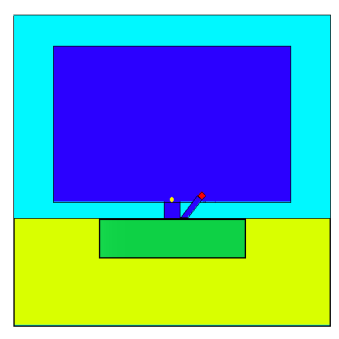
\includegraphics[width=0.7\textwidth]{images/sabatGeometry.png}
	\caption{Геометрія проекту SABAT} 
	\label{ris:SabatG}	
\end{figure}

Геометрія яка використовувалась для набору спектрів зоображена на Рис. ~\ref{ris:Geometry}, довжина ребра кубу середовища 1 м., довжина ребра бічної поверхні мішені (Рис. ~\ref{ris:Geometry} - 3 ) 40 см., від мішені до чутливого об'єму детектора 30 см., від чуливого об'єму до джерела 30 см., (відстані задані не враховуючи зовнішній захист) матеріал середовища був взятий с запропонованою бази матеріалів Geant4 - "G4\_WATER". Джерело нейтронів поміщене в напрявляючий об'єм(Рис. ~\ref{ris:Geometry} - 1), який виготовлений з токого шару свинцю. Чутливий об'єм детектора поміщений у захист зі свинцю, бору, та алюмінія, направляючі об'єми заповнені повітрям(G4\_AIR)
\begin{figure}[hbt!]
	%\vspace{-10pt}
	\centering 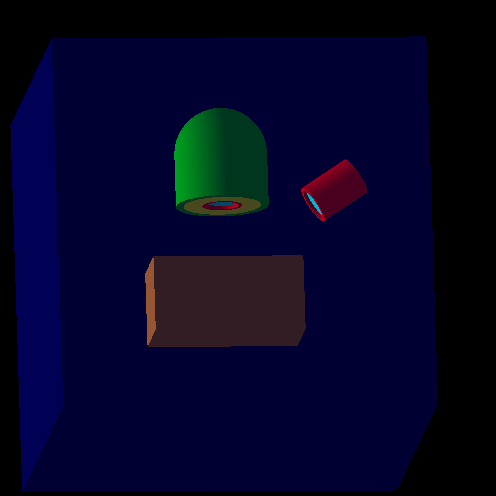
\includegraphics[width=0.7\textwidth]{images/geometryAll.png}
	\caption{Геометрія моделі, 1 - джерело і його направляючий об'єм, 2 - захист детектора та детектор, 3 - мішень} 
	\label{ris:Geometry}	
\end{figure}

Для спрощення моделювання точкове джерело нейтронів було розміщенне всередині набравляючого кооксіального об'єму Рис. ~\ref{ris:Geometry} (червоного кольору), під кутом для того щоб більша кількість нейтронів потрапляла в поверхню яка безпосередню знаходиться під чутливим об'ємом детектора 


\subsection{Чутливий об'єм детектора та захист}
	
	Для моделювання чутливого об'єму був обраний надчистий германій, з діаметром 60.6 міліметрів, та довжиною 56.7 міліметрів. Рис. ~\ref{ris:s_detector_volume} 	
	\begin{figure}[hbt!]
		%\vspace{-10pt}
		\centering 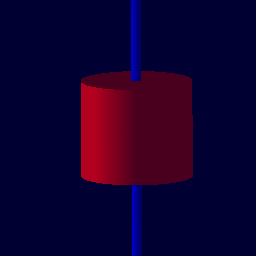
\includegraphics[width=0.7\textwidth]{images/sDetector158cm3.png}
		\caption{Форма чутливого об'єму} 
		\label{ris:s_detector_volume}	
	\end{figure}

	Детектор буде розміщенний поряд з джерелом нейтронів високих енергій, 14.5 МеВ. Тому детектор був розміщений у трьох шаровий захист. Рис. ~\ref{ris:s_detector_P}	
	\begin{figure}[hbt!]
		%\vspace{-10pt}
		\centering 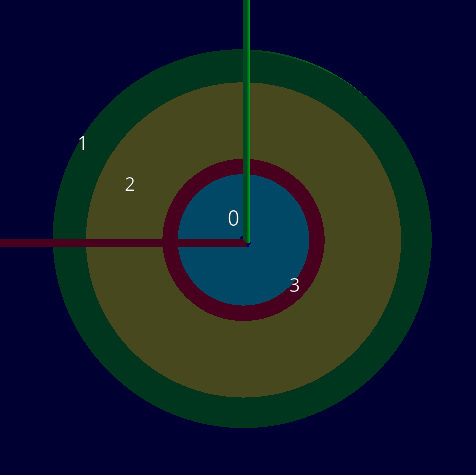
\includegraphics[width=0.7\textwidth]{images/dectorPrt.png}
		\caption{Захист детектора, Al - 1 (зелений) товщина 2 см., B - 2 (жовтий) товщина 5 см., Pb - 3 (червоний) товщина 1 см. 0 (Блакитний) шар повітря} 
		\label{ris:s_detector_P}	
	\end{figure} 

	В захисті використовується Бор для поглинання теплових нейтронів, так як вся детекторна система буде знаходитися під водою, то нейтрони від джерела будуть втрачати енергію при пружному розсіянні на водню. 
	
	Для поглинання теплових нейтронів перед чутливім об'ємом детектора був обраний $B^{10}$. Використовується в ПВЕЛ-ах для контролю кількості теплових нейтронів в активній зоні реакторної установки ВВЕР. 
	$B^{10} ( n, \alpha \gamma)Li_3^7$, Переріз захоплення нейтрона $B^{10} \ \sigma = 3380$ барн.
	$E_\gamma$ = 480 кеВ, реація з вильотом $\gamma$ - кванту протікає з ймовірністю 94\%.
	
	Для зовнішнього корпусу захисту чутливого об'єму використовувався $Al^{26}$ - товщиною 1 см на Рис. ~\ref{ris:s_detector_P} - зоображений зеленим кольором 
	
	За приклад було взято детектор N21879A виробника від ORTEC AMETEK, параметри розмірів були взяті від офіційного дестрибютера.
	
\subsection{Код моделі}
Цілью було написати максимально зручний код для набору спектрів за різних умов та на різних мішеннях, тому були створені абстрактні класси для створення геометричних об'єктів. Для зручності створення матеріалів були створенні структури. 
Та для пришвидшення роботи були всі можливі константи ініціалізувалися на етапі компіляції. Для полегшення контролю над пам'яттю використовувалися розумні вказівники С++ 14 стандарту. Архітектура коду моделювання зоображена на Рис. ~\ref{ris:s_classDiagram} 
\begin{figure}[hbt!]
	%\vspace{-10pt}
	\centering 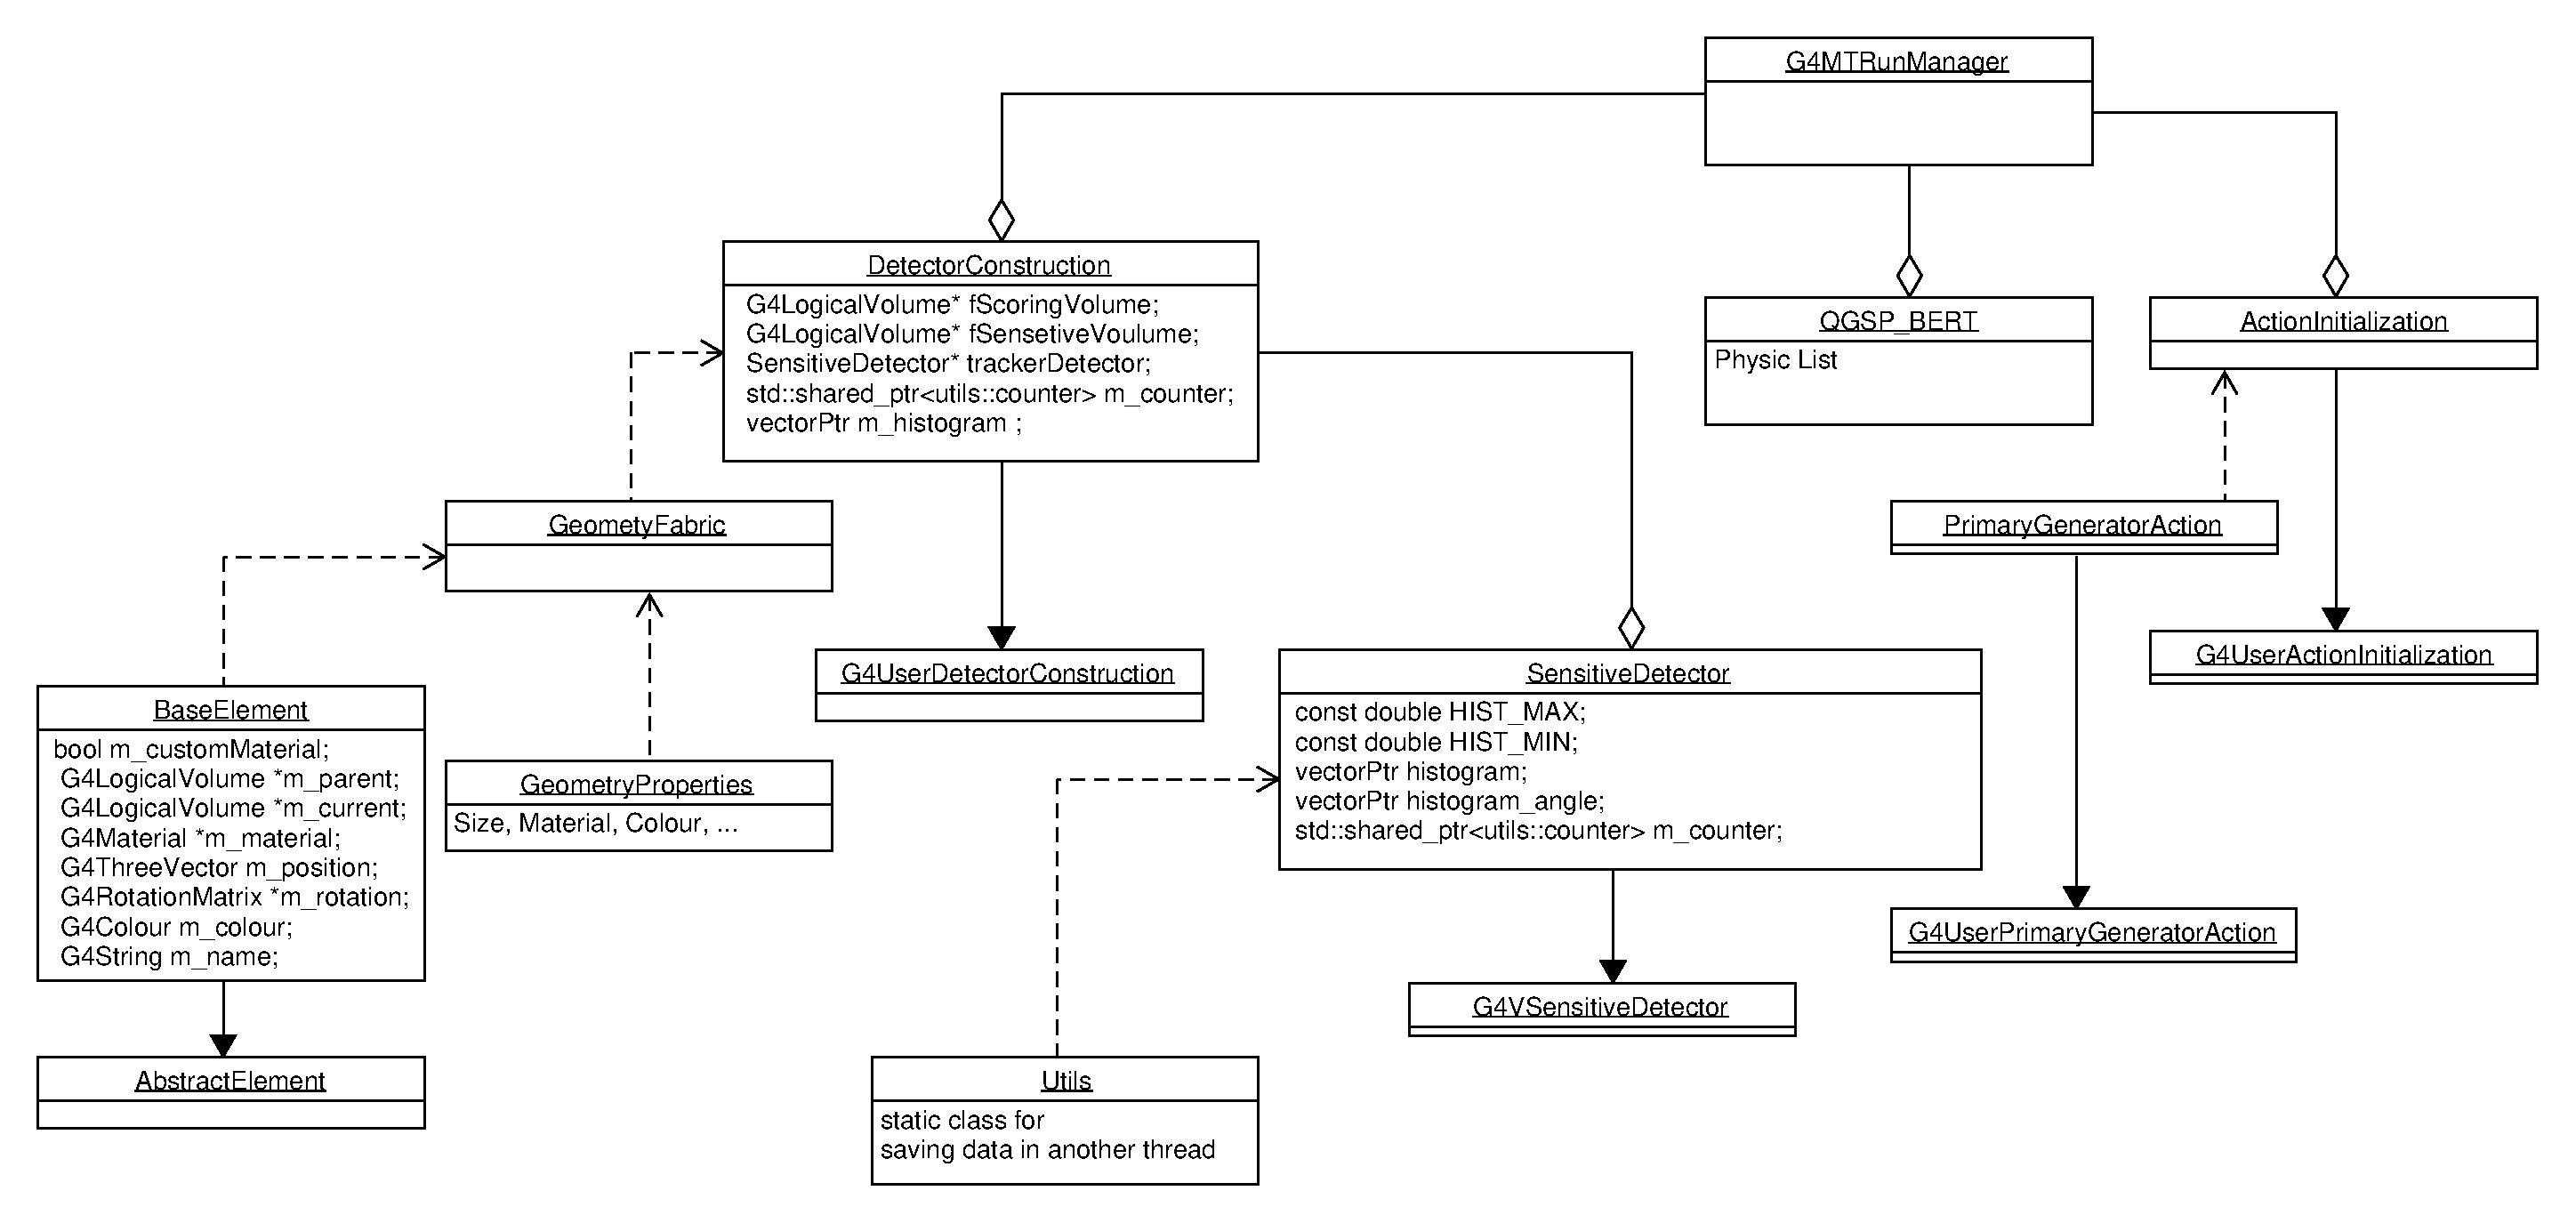
\includegraphics[width=1\textwidth]{res/classDiagram.pdf}
	\caption{Діаграма класів коду моделі} 
	\label{ris:s_classDiagram}	
\end{figure} 
Проаналізувавши різницю між двома фізичними моделями $QGSP\_BERT\_HP$ та $QGSP\_BERT$, для проведення моделювання була обрана $QGSP\_BERT$ - так як на данному єтапі вона виявилась більш підходящою, через вищу продуктивність.
	
\newpage 
\section{Розділ 3}
\setcounter{figure}{0}
\subsection{Опис обробки спектру}

В результаті моделювання, чутливим об'ємом набирались апаратні спектри, для чутливого об'єму було встановленно 16384 біни. Далі для наближення спектру до реального, була проведенне його сглажування за наступної формулою $\Delta{E} = 2.36 \sqrt{F  \frac{w}{E}}  w$, $\Delta{E}$ - енергія на один бін, F - Фано фактор, w - кількість енргії на утворення пари, та пронормований на кількість нейтронів з джерела. Так як для спрощення побудови джерела в моделі, використовувалась спрощенна геометрія, а генерація нейтронів відбувалась майже строго у заданому напрямку. Так як джерело нейтронів вважалося ізотропним, то загальна кількіть частинок розраховувалась наступною формолую $ 4 \pi n = N$, де $N -$ це загальна кількість чатсинок. В моїй роботі для зглажування спектру були взяті наступні параметри Табл. ~\ref{tabl:Param}
\begin{table}[h]
	\centering
	\begin{tabular}{|c|c|c|} 
		\hline
		Параметр & Значення &  Розмірність \\
		\hline
		$F$ & 0.13 & - \\
		\hline
		$w$ & 3.62 & eV \\		
		\hline
	\end{tabular}
	\caption{Таблиця значень для уширення піків} 
	\label{tabl:Param}
\end{table}
\begin{figure}[hbt!]
	%\vspace{-10pt}
	\centering 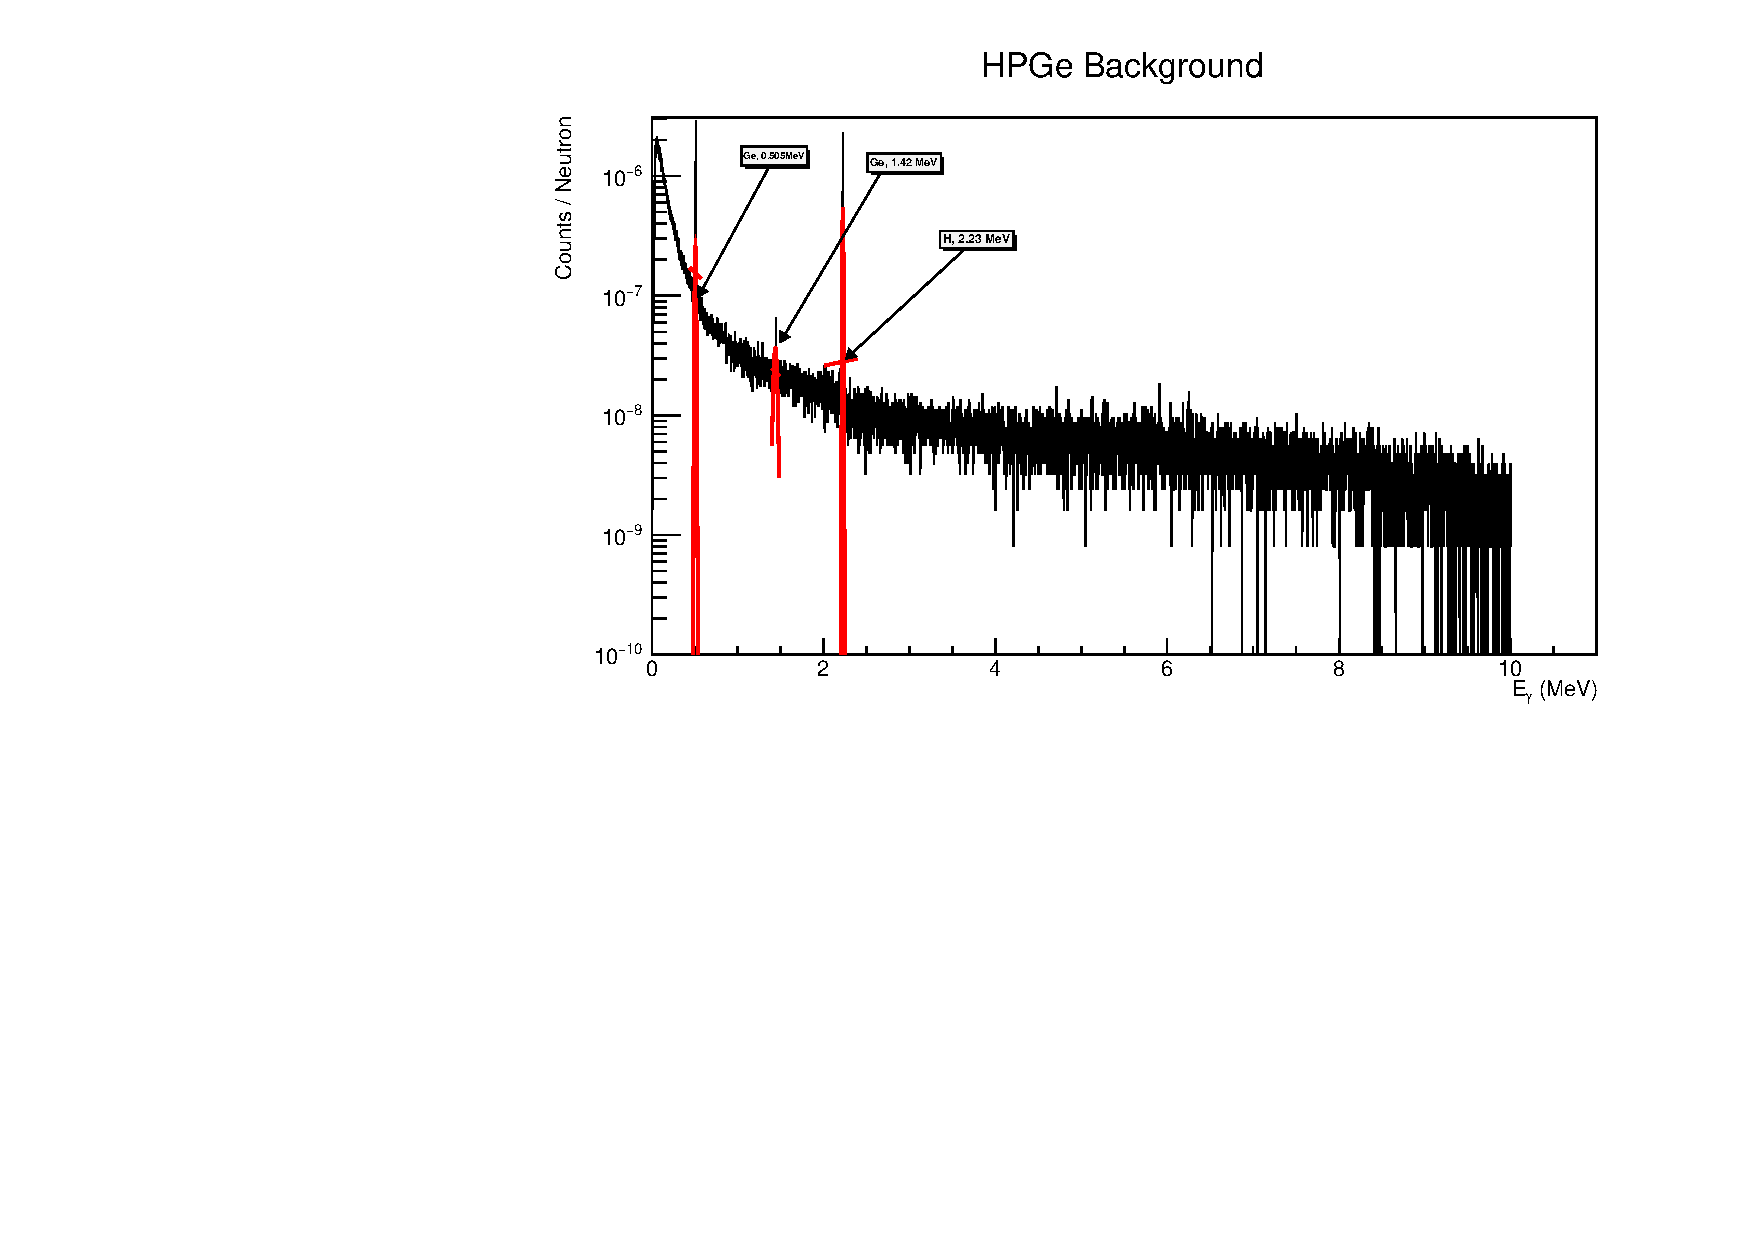
\includegraphics[width=1\textwidth]{res/background.pdf}
	\caption{Фон} 
	\label{ris:FonPicks}	
\end{figure} 

Фон Рис. ~\ref{ris:FonPicks} набирався за тих тої самої геометрії Рис. ~\ref{ris:SabatG}, але за відсутності мішені(коричневий паралелепіпед), У фоні були проаналізовані наступні три піки: H з $E_\gamma = 2.23 MeV$, та два піки які отримались за рахунок захоплення теплових нейтронів $Ge$ з $E_\gamma = 0.505MeV$, $E_\gamma = 1.42 MeV$ - це означає що данної геометрії частина нейтронів від джерела проходячи через захист потрапляє в чутливий об'єм детектора, та призводить до його руйнації. Данні піки відповідають пікам $Ge^{72}(n, \gamma)Ge^{73}$ - реакції з нейтронами енергій близькими до теплових - $E_n = 0.025eV$. $Ge^{72}$ - основний ізотоп Ge, і саме він використовувася в основі чутливого об'єму.
\begin{table}[h]
	\centering
	\begin{tabular}{|c|c|c|c|} 
		\hline
		$E_{\gamma}$, MeВ & $\Delta{E}$, МеВ & $I = I_{\gamma} / I_{b}$ & $\Delta{I}$\\
		\hline
		0.505 & 0.008 & 12 & 3 \\
		\hline
		1.420 & 0.004 & 20 & 4 \\	
		\hline
		2.230 & 0.003 & 22 & 4 \\	
		\hline
	\end{tabular}
	\caption{Фонові піки} 
	\label{tabl:ResultsBackground}
\end{table}

\subsection{Валідація моделі}

	Для підтвердження можливості проведення наборів на моїй моделі був набраний спектор для Гірчичного газу ($C_4H_8Cl_2S$). Рис ~\ref{ris:MustBackAllLogSm}. Та порівняний з отриманим спектром набраним задопогою коду для моделювання MCNP в проекті SABAT.
	\begin{figure}[hbt!]
		%\vspace{-10pt}
		\centering 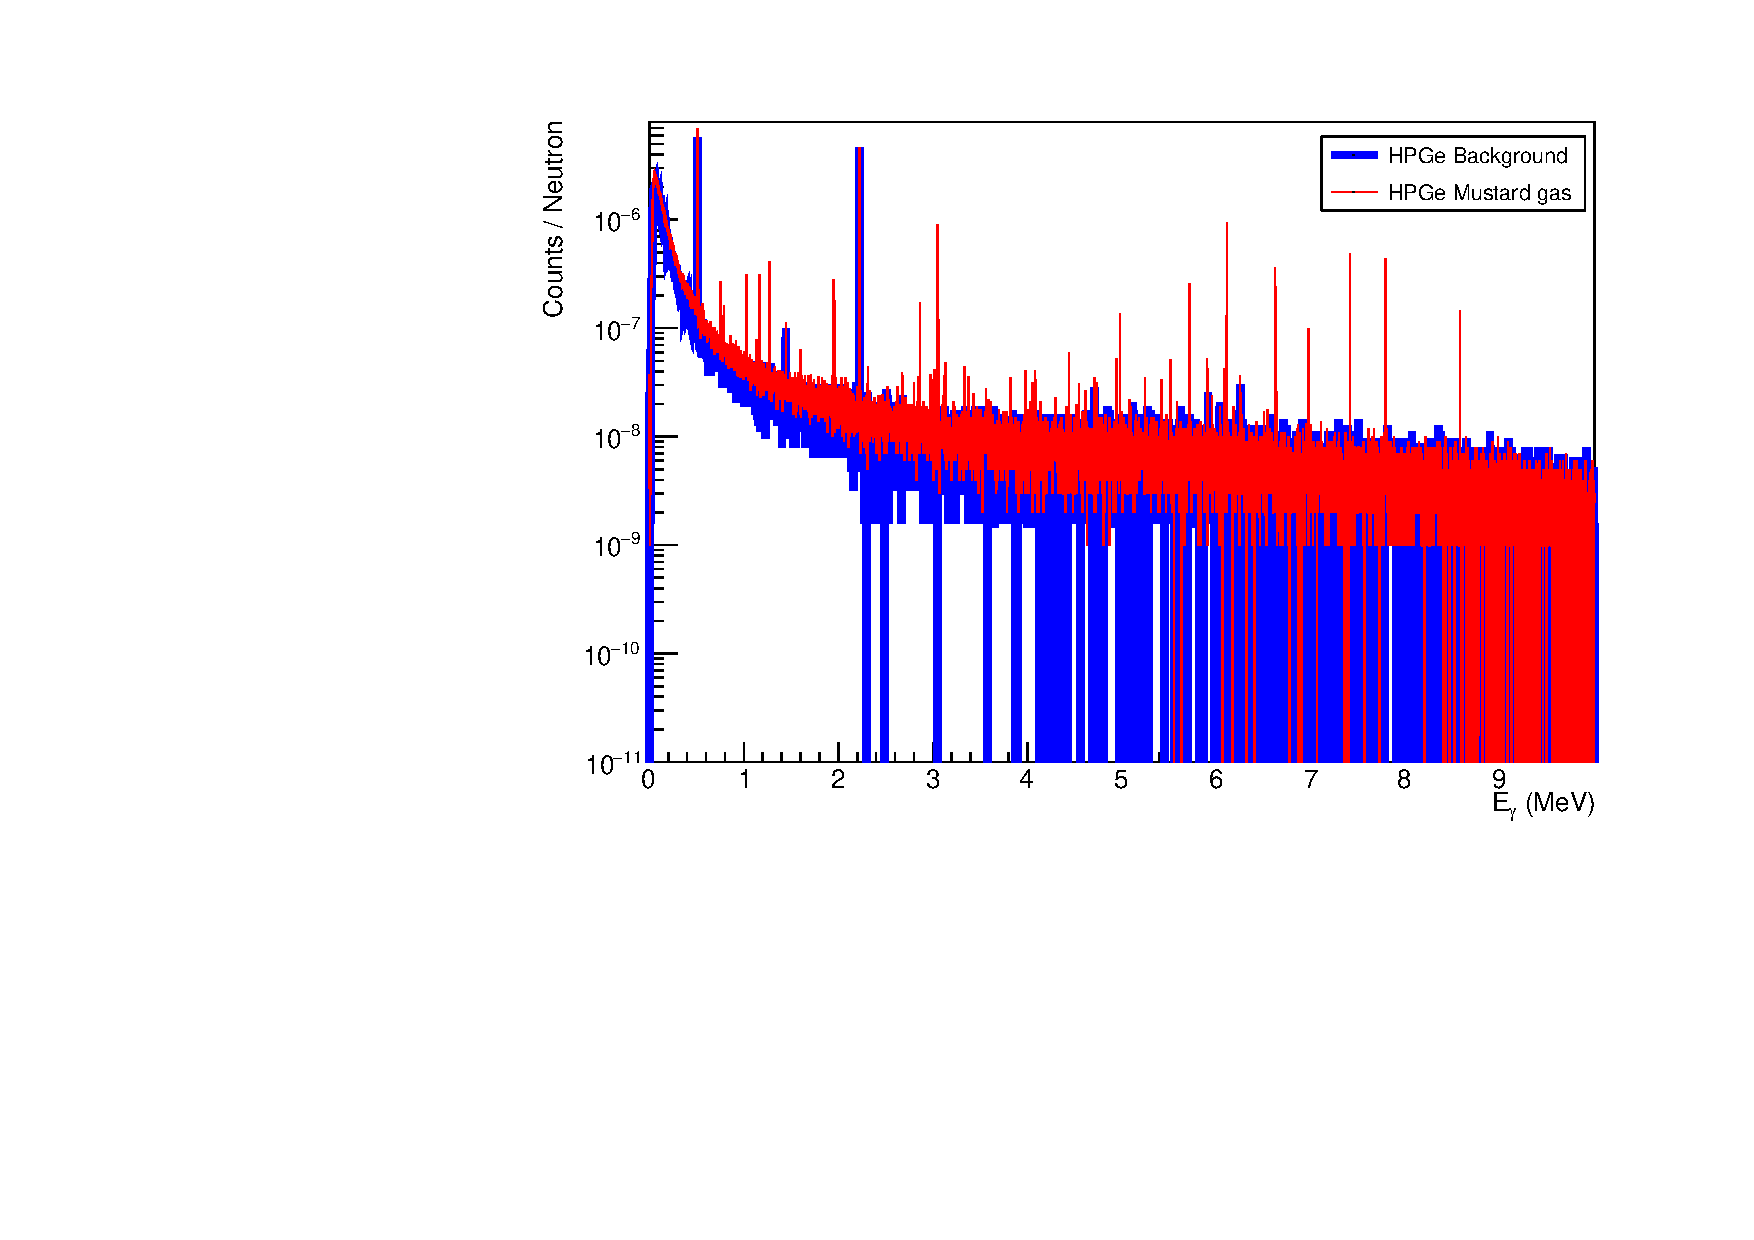
\includegraphics[width=1\textwidth]{res/smMustFonAll.pdf}
		\caption{Червоним - представлений спектор для Гірчичного газу. Синім - фону} 
		\label{ris:MustBackAllLogSm}	
	\end{figure} 
	Це спектор набирався для валідації моделі - тому до уваги бралися лише ті піки, які були вказані в проекті SABAT. Табл. ~\ref{tabl:ResultsMustard}
	\begin{table}[h]
		\centering
		\begin{tabular}{|c|c|c|c|c|} 
			\hline
			$E_{\gamma}$, MeВ & $\Delta{E}$, МеВ & $I = I_{\gamma} / I_{b}$ & $\Delta{I}$ & Елемент\\
			\hline
			0.79 & 0.008 & 12 & 3 & Cl\\
			\hline
			1.165 & 0.004 & 20 & 4 & Cl \\	
			\hline
			1.95 & 0.003 & 22 & 4 & Cl \\	
			\hline		
			4.44 & 0.003 & 22 & 4 & C \\	
			\hline
			7.41 & 0.003 & 22 & 4 & Cl\\	
			\hline
			7.78 & 0.003 & 22 & 4 & Cl\\	
			\hline			
			8.58 & 0.003 & 22 & 4 & Cl\\	
			\hline
		\end{tabular}
		\caption{Піки гічичного газу - $C_4H_8Cl_2S$} 
		\label{tabl:ResultsMustard}
	\end{table}
	
	\begin{figure}[hbt!]
		%\vspace{-10pt}
		\centering 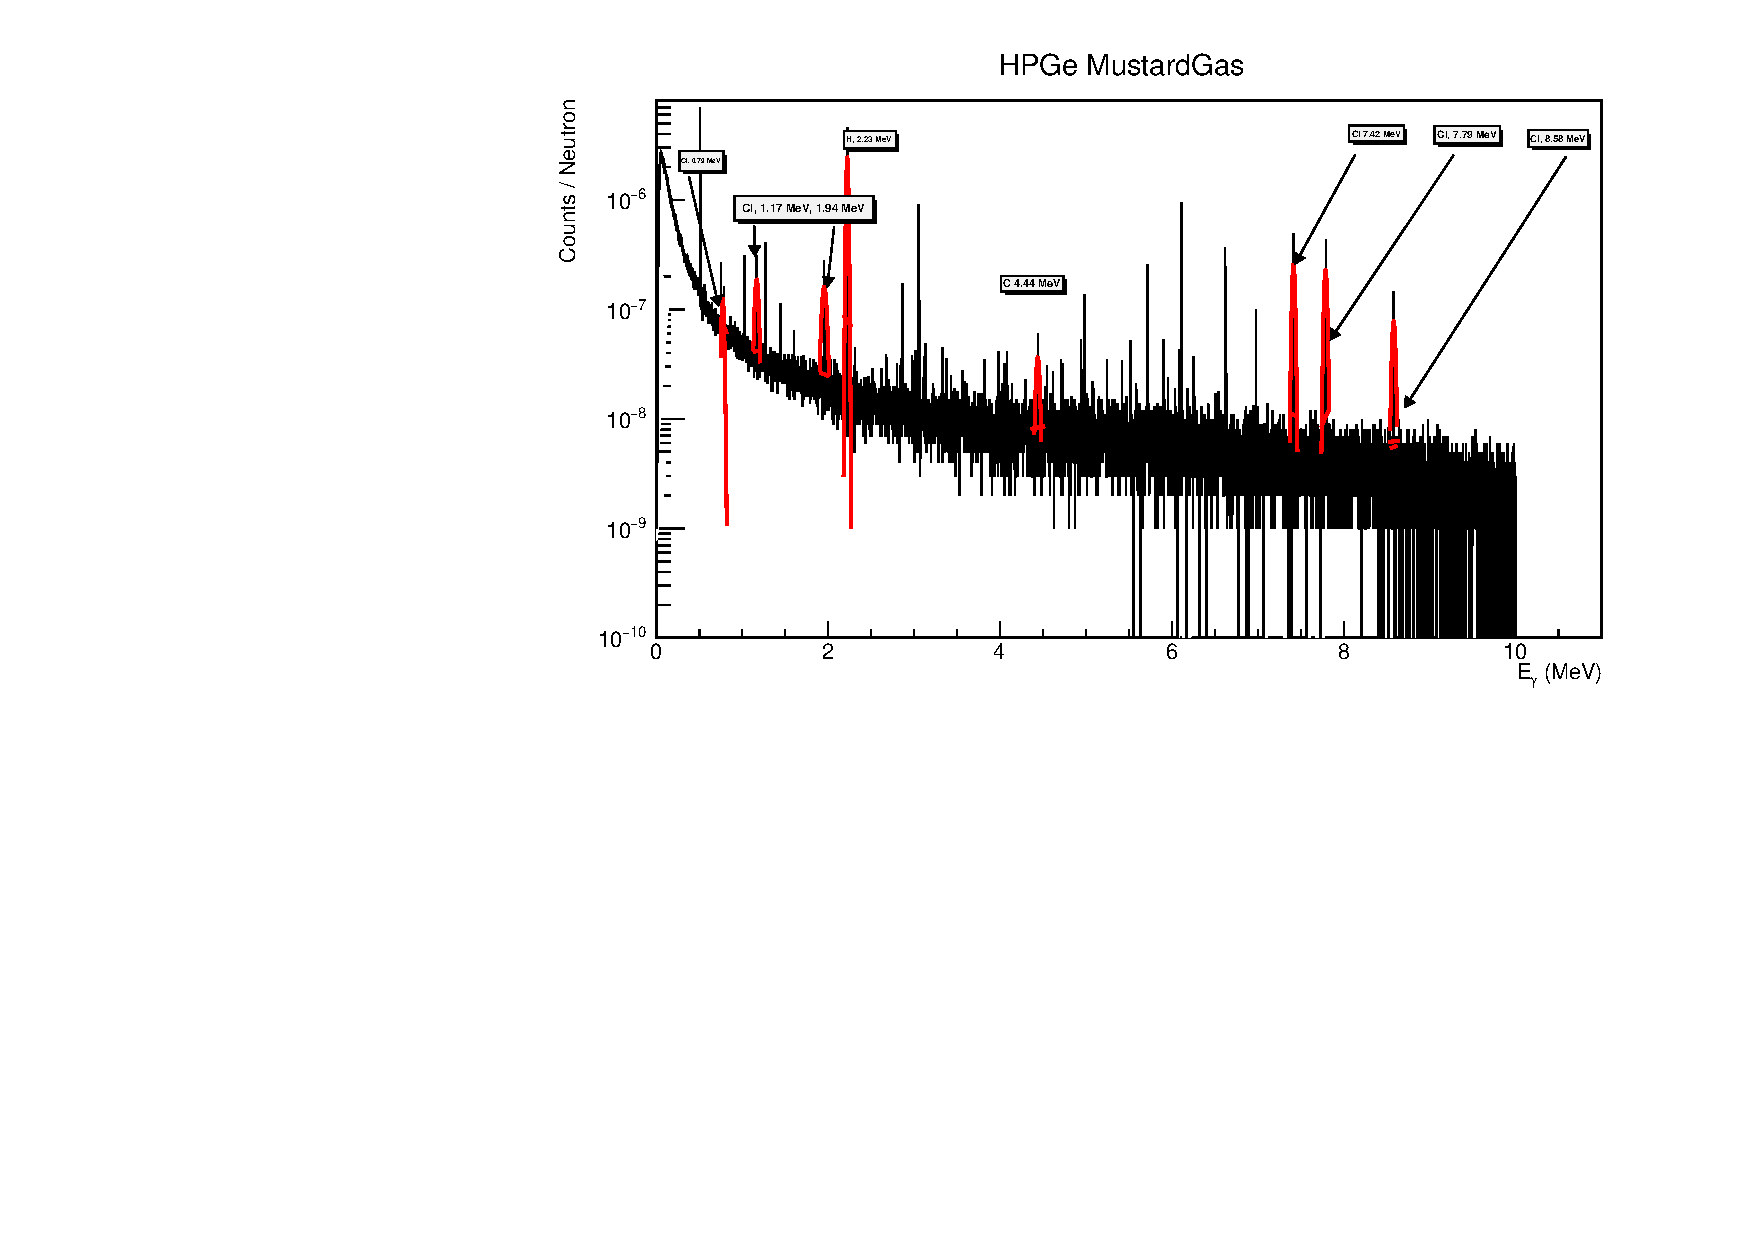
\includegraphics[width=1\textwidth]{res/mustard_gas.pdf}
		\caption{Ініціалізвція піків, Cl, H, C - в спектрі гірчичного газу} 
		\label{ris:mustard}	
	\end{figure} 
	
\subsection{Дослідження $(n, \gamma)$ реакцій, Au та Cu} 
$Au^{197}(n,\gamma)Au^{198}$ - реакція захоплення нейтронна, переріз захоплення нейтронів в залежності від енергії зоображено на Рис.~ \ref{ris:AuSigma}.
\begin{figure}[hbt!]
	%\vspace{-10pt}
	\centering 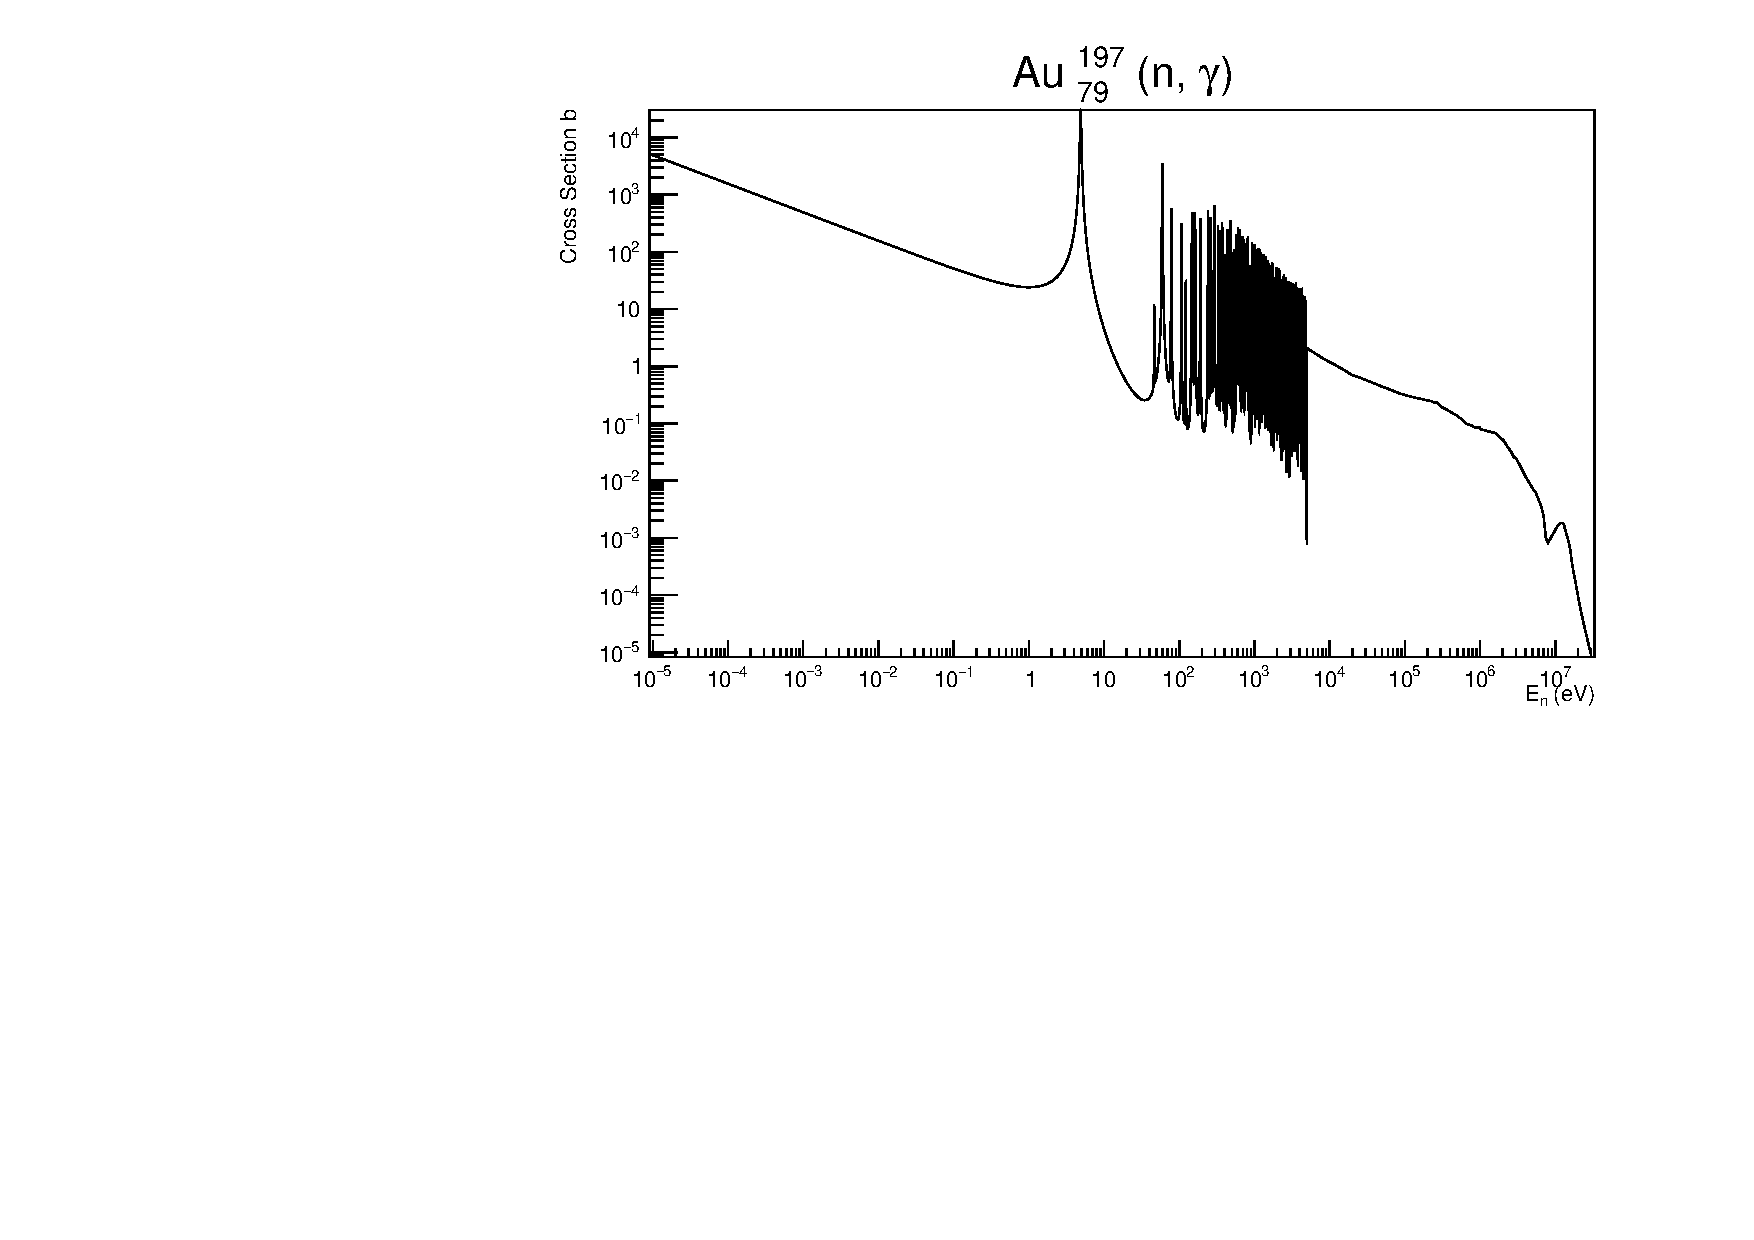
\includegraphics[width=1\textwidth]{sigma/Au197Sigma.pdf}
	\caption{Залежність захоплення нейтрона від енергії нейтронів в реакціїї  $Au^{197}(n,\gamma)Au^{198}$} 
	\label{ris:AuSigma}	
\end{figure} 

$Au^{198} $ - ізотоп, має 2 - рівні в результаті розпаду з яких випромінються гамма кванти, $T_{1/2} = 2.6$ днів. На Рис. \ref{ris:Au198Level12-} зоображенно перехід з збудженного $J\pi$ 12- на $J/\pi$ 2- з якого у данного ізотопа відбувається $\beta^-$ розпад до стабільного $Hg^{198}_{80}$.

$Hg^{198}$ - має два збудженні рівні $J\pi$ 2+ - перехід з  в основний стан відбуваеться з випромінення $\gamma$-кванту $E_\gamma=1087keV$, каскадний періхід є осноним с способ переходу на стабільний рівень $Hg^{198}$, відбувається з випромінення двох $\gamma$-квантів $E_\gamma$ = 675 кеВ та $E_\gamma$ = 411 кеВ. 

На Рис. ~\ref{ris:AuSigma} - гарно видно що є резонансна область поглинання нейтронів розтягується до декількох кеВ. 
\begin{table}[h]
	\centering
	\begin{tabular}{|c|c|c|c|c|} 
		\hline
			$E_{n}$, eВ&$E_{\gamma}$, кеВ & $\Delta{E_{\gamma}}$, кеВ & $I_{\gamma} / 100_n$ & $\Delta{I}$ \\
		\hline
		4.9 & 6252.6 & 0.7 & 40.0 & 1.6 \\
		\hline
		4.9 & 6457.8 & 0.7 & 20.4 & 0.5\\	
		\hline
		4.9 & 5710.7 & 0.7 & 10.1 & 0.7 \\	
		\hline	%60.        6061.3      0.9        16.2   -01  1.5 	
		60 & 6061.3 & 0.9 & 16.2 & 1.5 \\	
		\hline % 5710.7      0.7        16.0   -01  1.5   -01
		60 & 5710.7 & 0.7 & 16.0 & 1.5 \\	
		\hline % 78.        4958.2      1.0        10.5   -01  0.6   -01
		78 & 4958 & 1.0 & 10.5 & 0.6\\	
		\hline% 107.       5808.2      0.9        17.3   -01  1.0   -01
		107 & 5808.2 & 0.9 & 17.3 & 1.0 \\	
		\hline
	\end{tabular}
	\caption{$E_\gamma$, для нейтронів з енргіями поблизу резонансної області для $Au^{197}$} 
	\label{tabl:AuNeutronAbsorption}
\end{table}

В реакція $Cu^{64}(n, \gamma)Cu^{65}$ переріз захоплення теплового нейтрона $\sigma$ = $2.1 \times 10^3 \pm \ 1.9 \times 10^3$ барн. $Cu^{65}$ - стабільний елемент. $Cu^{65}(n,\gamma)Cu^{66}$.
\begin{figure}[hbt!]
	%\vspace{-10pt}
	\centering 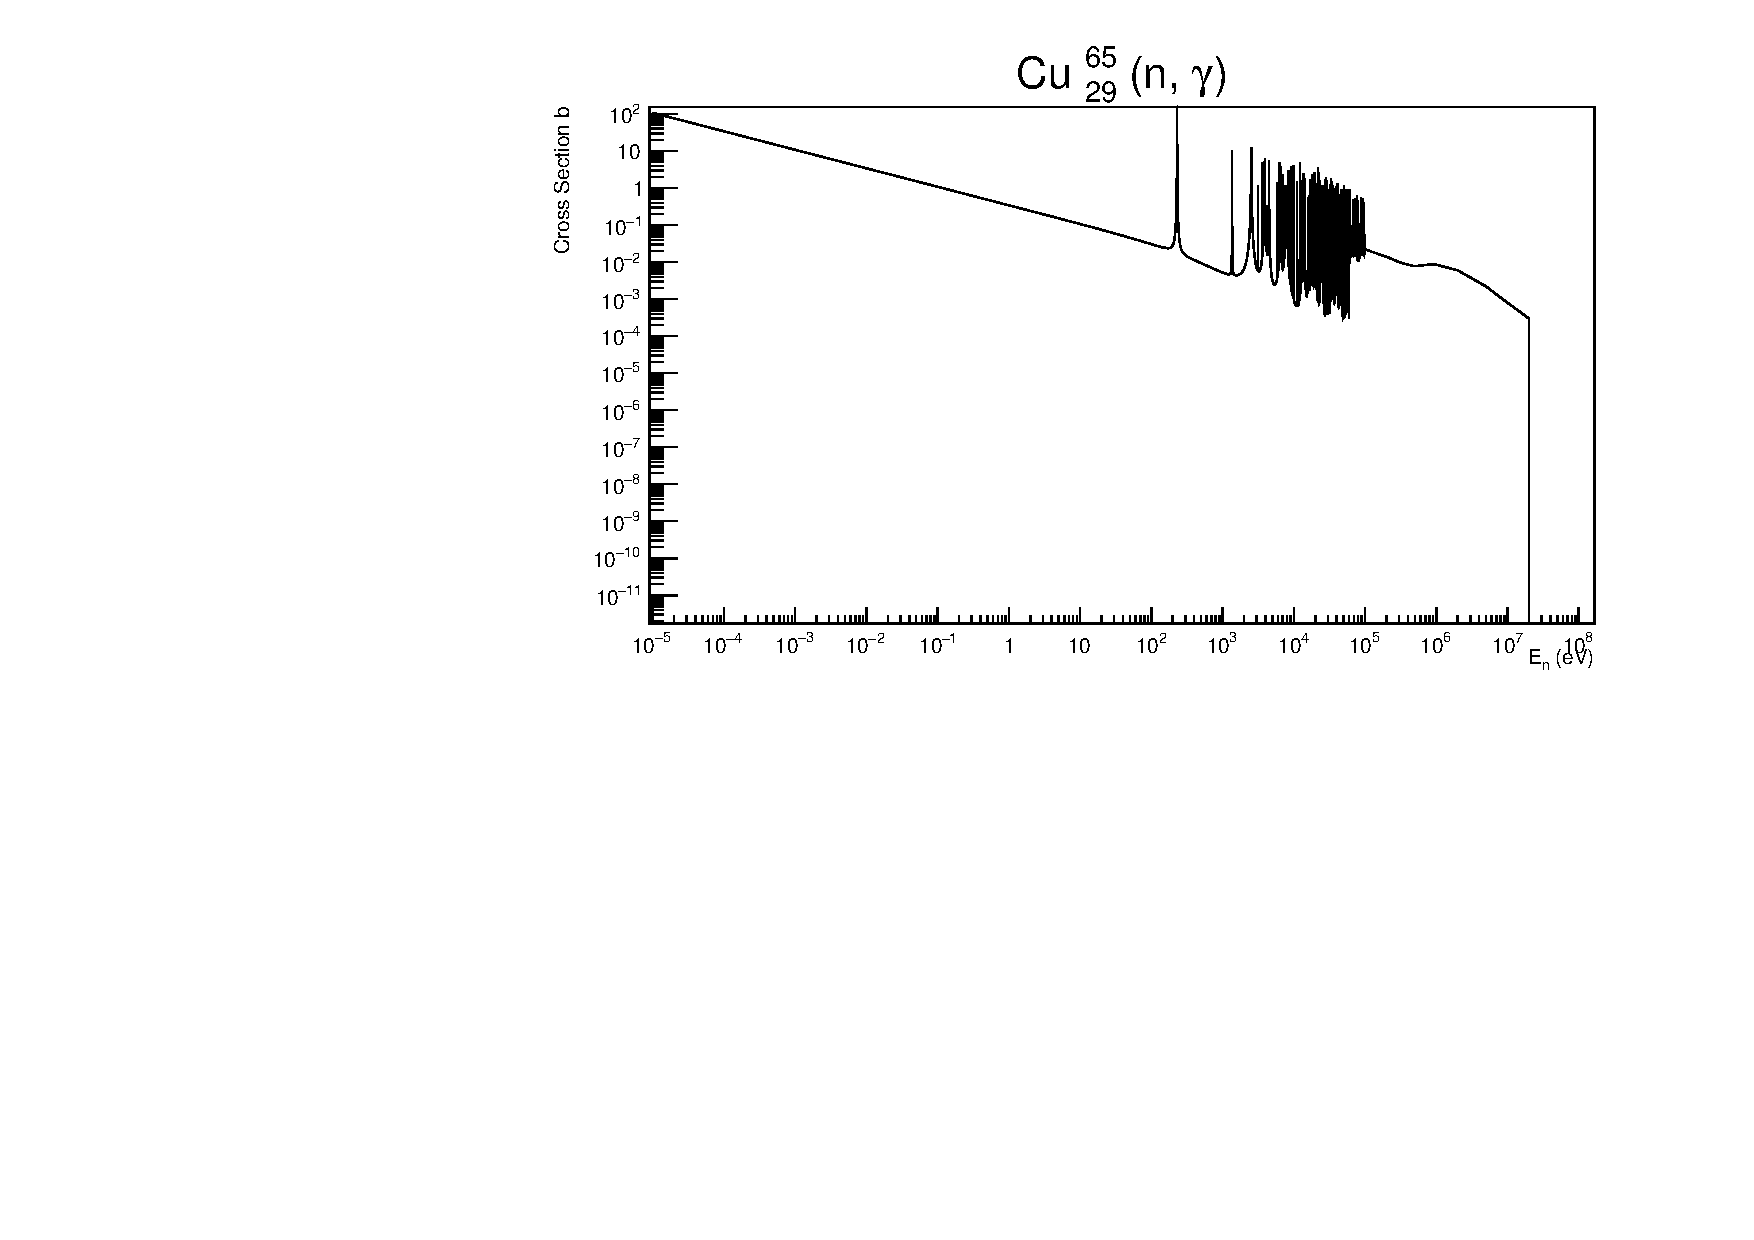
\includegraphics[width=1\textwidth]{sigma/Cu65Sigma.pdf}
	\caption{Залежність захоплення нейтрона від енергії нейтронів в реакціїї  $Cu^{65}(n,\gamma)Cu^{66}$} 
	\label{ris:CuSigma}	
\end{figure} 
Для данного изотопу спостерігається існування резонансної області в діапазоні десятків кеВ Рис. ~\ref{ris:CuSigma}. 
$Cu^{66}$ - не стабільний ізотоп, якому притаманний $\beta^-$ розпад в $Zn^{66}_{30}$, $T_{1/2} = 5.12$ хвилин. 
$Zn^{66}$ - стабільний ізотоп з основним рівнем $J\pi$ 0+. $\beta^-$ - розпад $Cu^{66}$ в основному відбуваеться у ставбільний стан, але є ймовірність розпаду на $J\pi$ 1+ рівень, з подальшим випромінення $\gamma$ - кванту з енергією $E_{\gamma} = 1039$ кеВ. Рис. ~\ref{ris:ZnLevels-}
\\
\subsection{Аналіз спектрів $Ag_3AuS_2$}
За матеріал було обрано ютенбогардтит $Ag_3AuS_2$ - родовища з данними мінералами були знайдені на камчатці поблизу побережжня. Данний мінерал відноситься до рідкисних золотоносних руд, зустрічаеться в природі у твердому стані. Був знайдений на Камчатських родовищах. Рис. ~\ref{ris:Ag3AuS2Fon}	
\begin{figure}[hbt!]
	%\vspace{-10pt}
	\centering 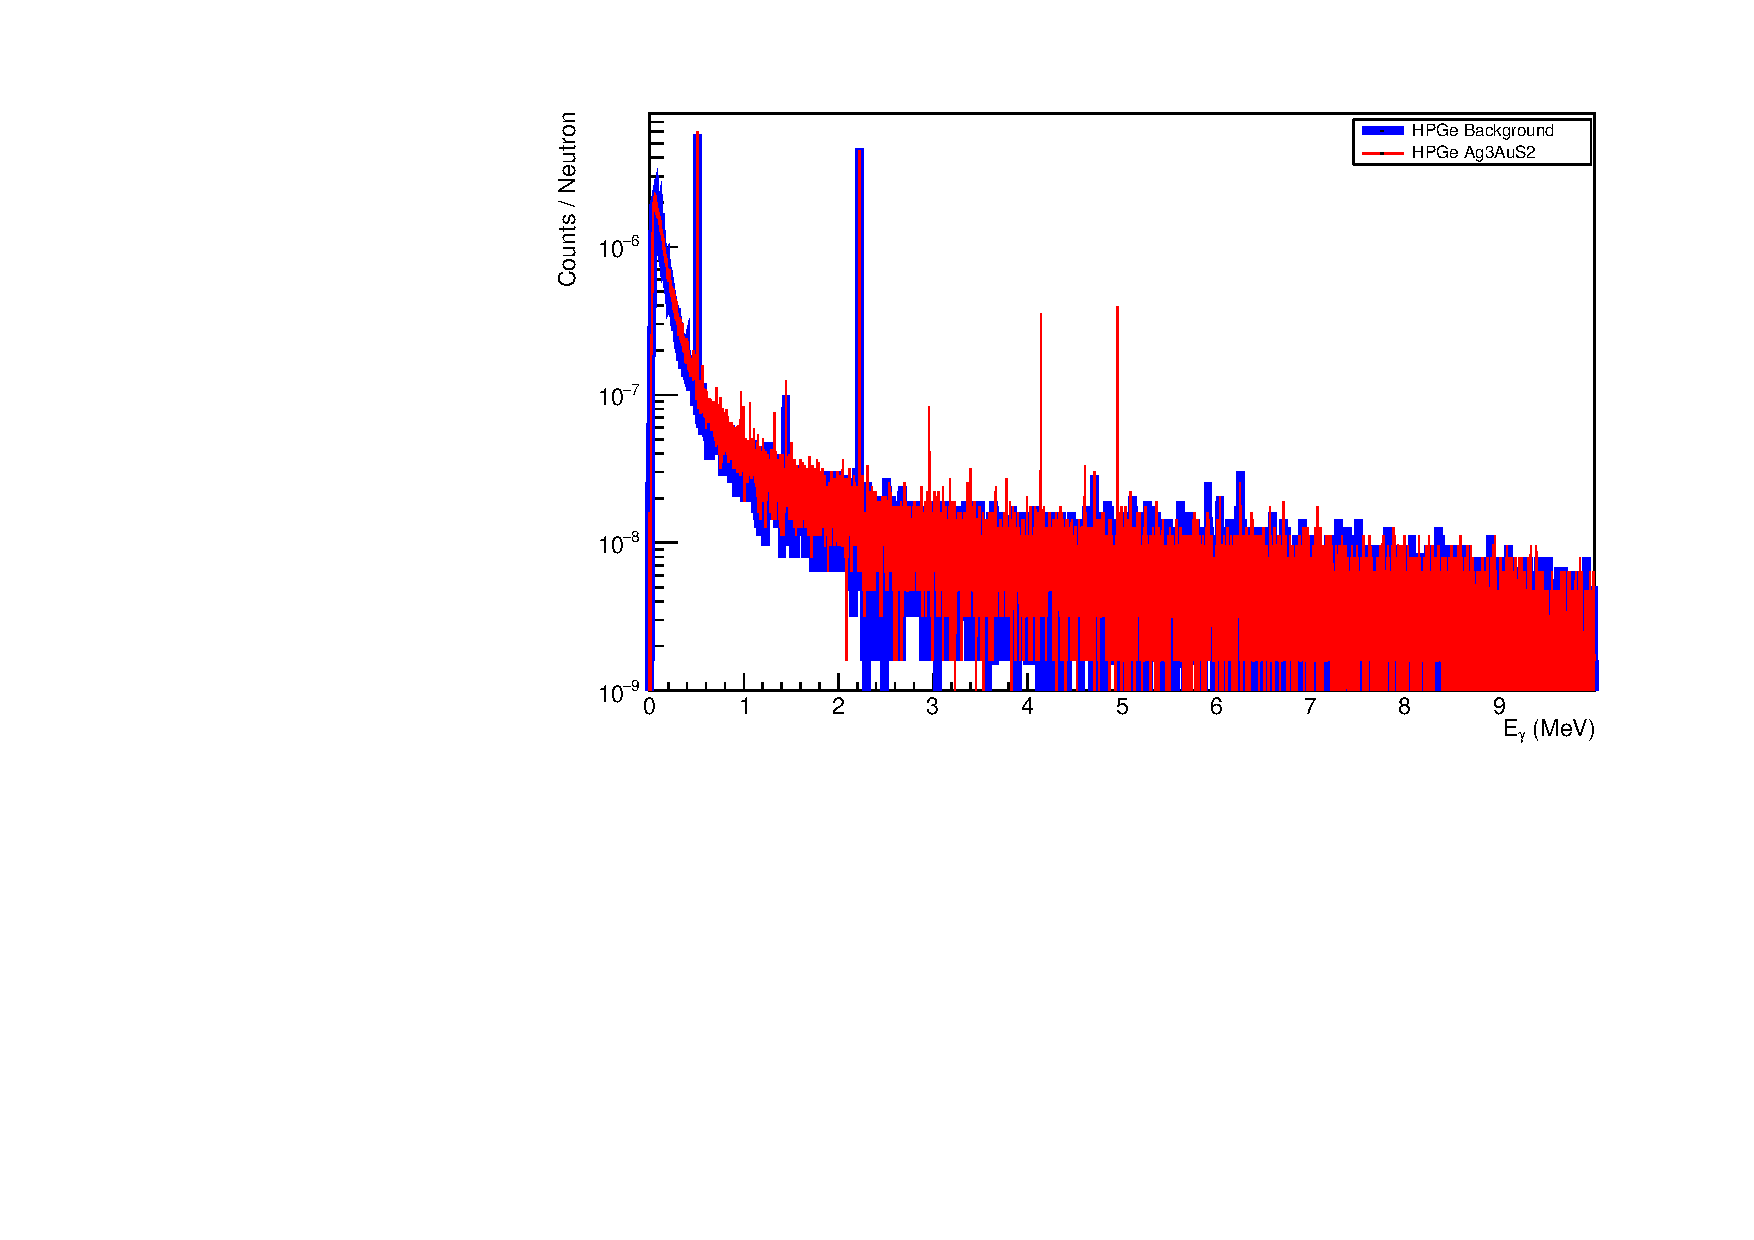
\includegraphics[width=1\textwidth]{res/auFonAllLog.pdf}
	\caption{Червоним - представлений спектор для $Ag_3AuS_2$. Синім - фону} 
	\label{ris:Ag3AuS2Fon}	
\end{figure} 	
Данний спектор і фон були набрані при опроміненні нейтронами з джерела максимальної енергією 14.5 МеВ
Для порівняння було проведенно опромінення за допомгою нейтронів енергією 8.5 та 2.8 МеВ. Рис. ~\ref{ris:Ag3AuS28_5MeV}	
В набраному спектрі при енергіях нейтронів з джерела 8.5 МеВ, були проаналізовані наступні піки
\begin{figure}[hbt!]
	%\vspace{-10pt}
	\centering 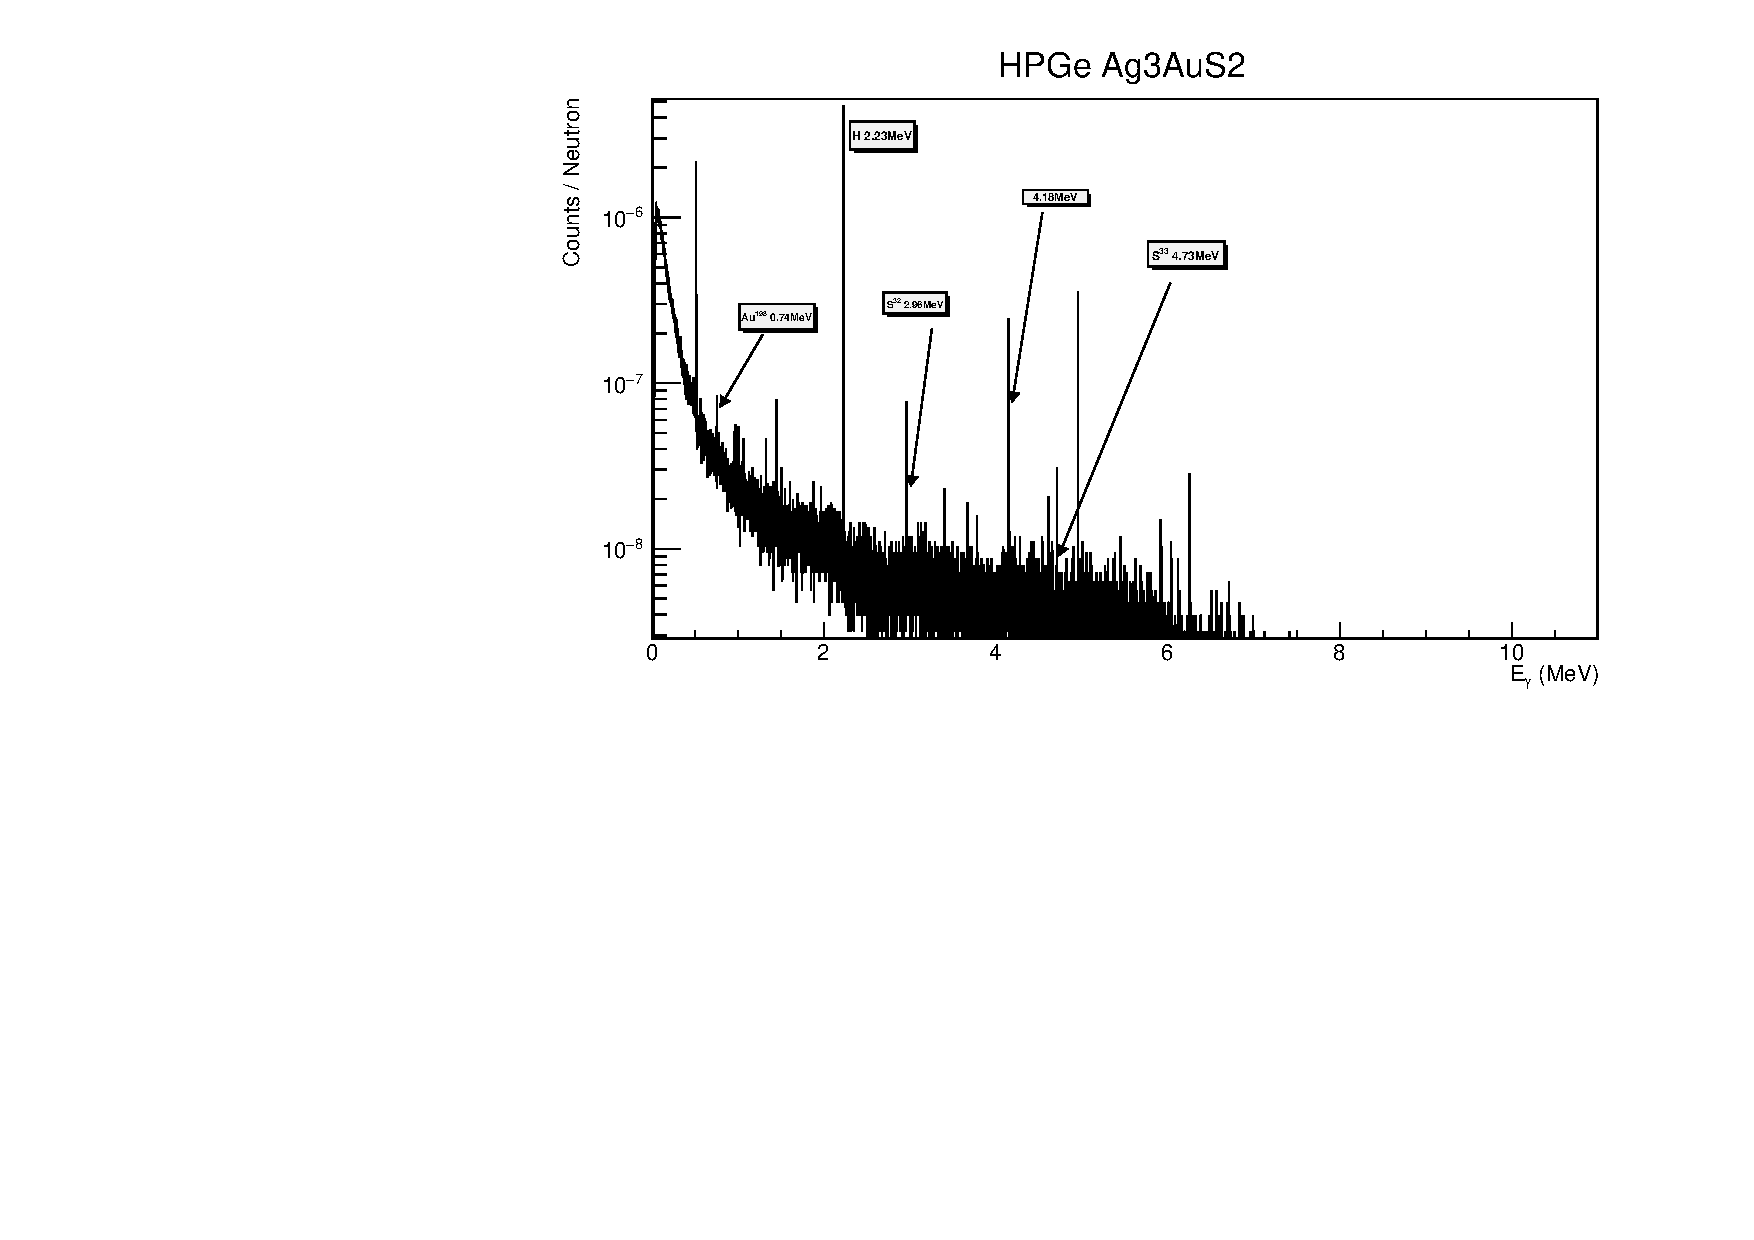
\includegraphics[width=1\textwidth]{res/Au_AnzSpectr.pdf}
	\caption{Спектор $Ag_3AuS_2$, $E_{n} = 8.5 MeV$ - енергія нейтронів з джерела}
	\label{ris:Ag3AuS28_5MeVPick}	
\end{figure} 
Для того щоб проаналізувати залежність можливості використання ізотопних джерел був набраний спектор, за енергій нейтронів 2.8 МеВ Рис. ~\ref{ris:Ag3AuS22_8MeV}

\subsection{Аналіз спектрів $CuFeS_2$}
	Данний мінерал являеться основною складовою мідної руди, спектор для нього представлений на Рис. ~\ref{ris:CuFeS_2Fon}
	\begin{figure}[hbt!]
		%\vspace{-10pt}
		\centering 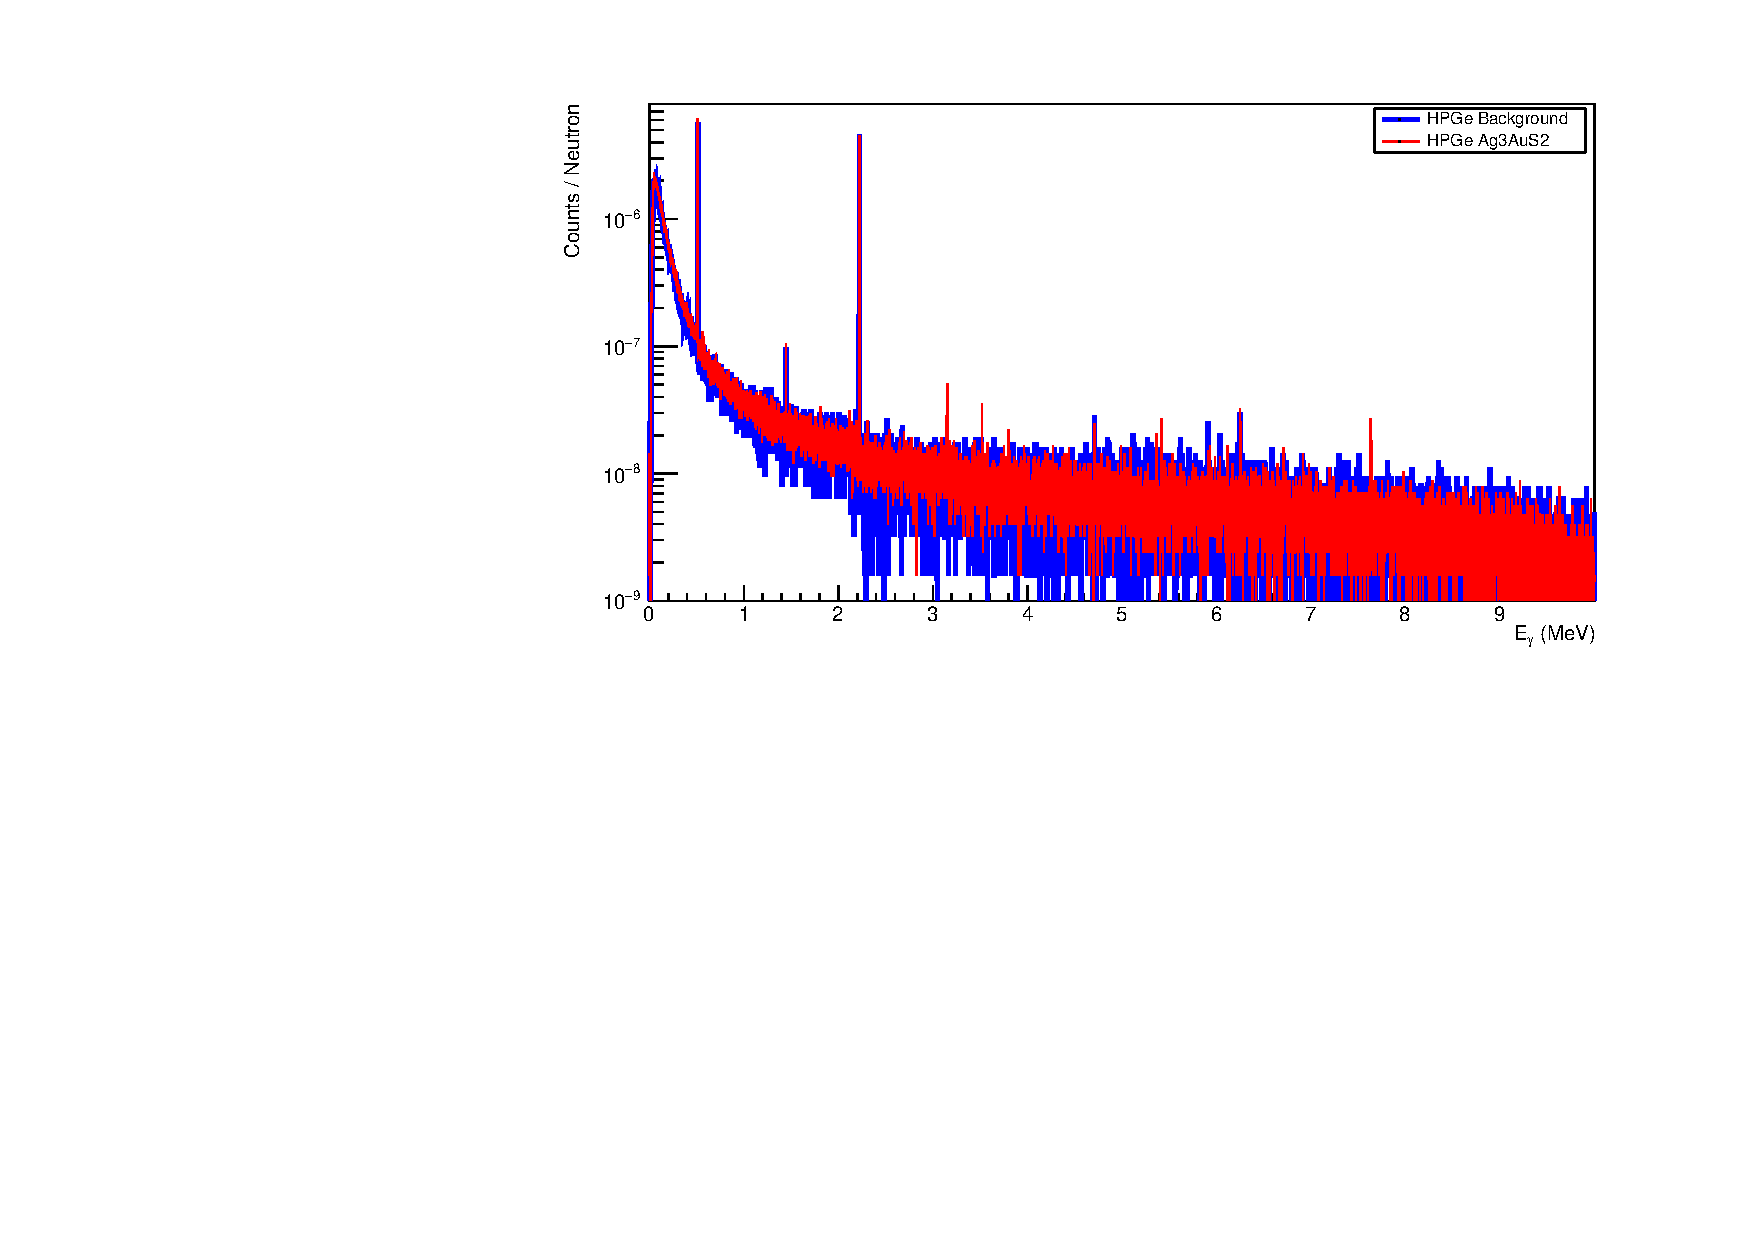
\includegraphics[width=1\textwidth]{res/smCuFeS2FonAll.pdf}
		\caption{Червоним - представлений спектор для $CuFeS_2$. Синім - фону} 
		\label{ris:CuFeS_2Fon}	
	\end{figure} 	
	В високо енергетичній частині спектру можна спостерігати пік для $S_2$
		
\subsection{Аналіз спектру $U^{238}$}
	<Мета набору> Було обрано збіднений уран, з наступним ізотопічним складом $99.27\% -\  ^{238}U$, $ 0.72\% - \  ^{235}U$, $ 0.005\% - \ ^{234}U$, У ході набору було отримано наступний спектор Рисю ~\ref{ris:poorU}
	\begin{figure}[hbt!]
		%\vspace{-10pt}
		\centering 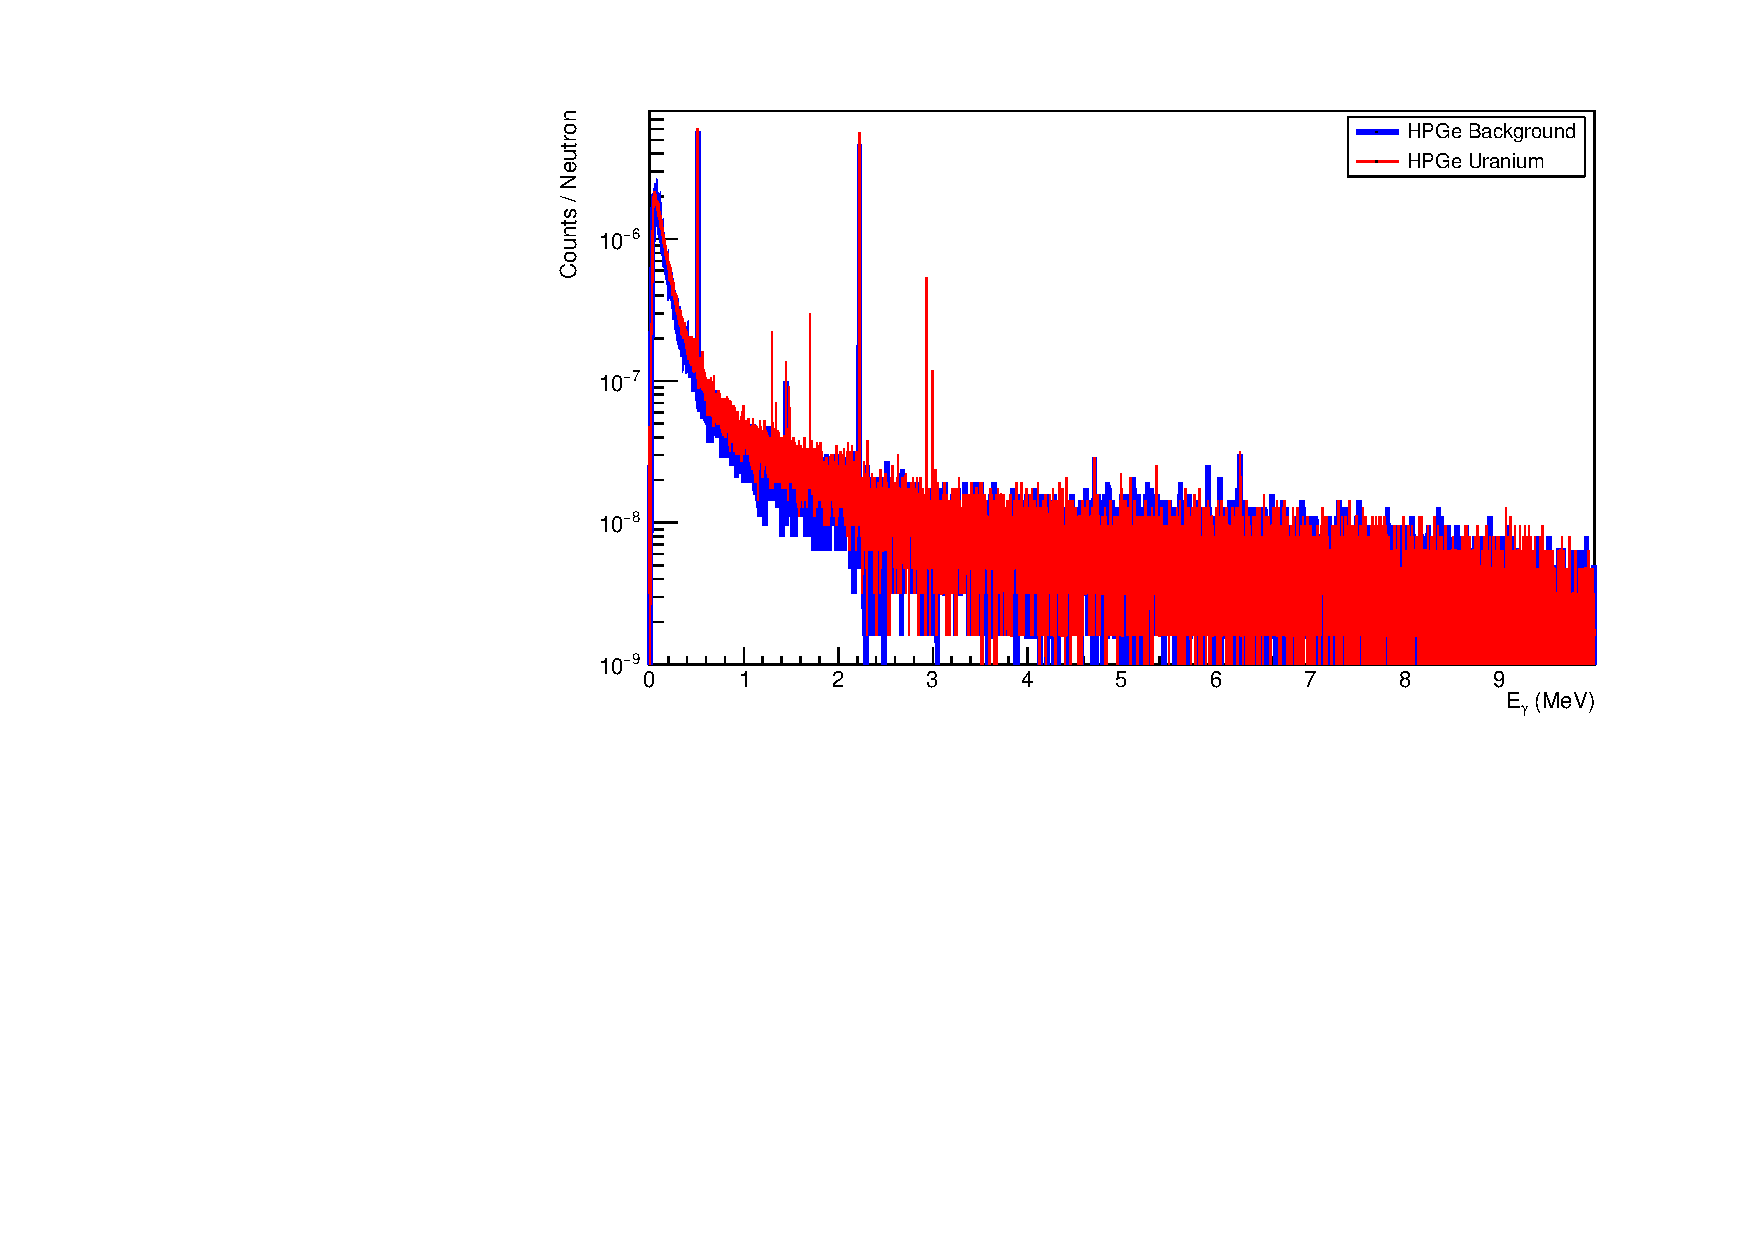
\includegraphics[width=1\textwidth]{res/poorUranium.pdf}
		\caption{Червоним - представлений спектор для $U^{238}$. Синім - фону} 
		\label{ris:poorU}	
	\end{figure} 	 
	На данному спектрі можна спостерігат
	
\newpage 
\section{Висновки}
\setcounter{figure}{0}
У роботі була змодельована спрощена версія системи яка дає змогу досліджувати, та індетифікувати речовини які знаходяться не лише на поверхні океанічного дна, при достатніх потоках нейтронів, та необхідного рельєфу.

Модель була успішно пройшла валідацію на спектрі для гірчичного газу з проекту SABAT. 

Проведння набору спетрів для нейтронів різних енергій дало, можливість виявити та зареєгіструвати недоліки данної моделі та геометрії. 

На данному єтапі було проведонно перевірку використання данної моделі для обмеженної кількості речовин. Та згідно з результату, подібна модель має можливість для застосування, для високо збагачених руд.

Встановленна відстань від джерела нейтронів до досліджуванної речовини може варіюватись і бути більшою за 30 см. - енергіях нейтронів 14 МеВ. Також було визначено що при використанні напівпровідникового детектора, відстань між джерелом та деетктором однозначно повинна бути більшою за 30 см. 

Використання захисту детектора з $B^{10}$ - є не достатньо єфективним. 

Також було встановленно що використання ізотопних джерел нейтронів є не доцільним 

\newpage 
\section{Додатки}
\setcounter{figure}{0}
\begin{figure}[h!]
	%\vspace{-10pt}
	\centering 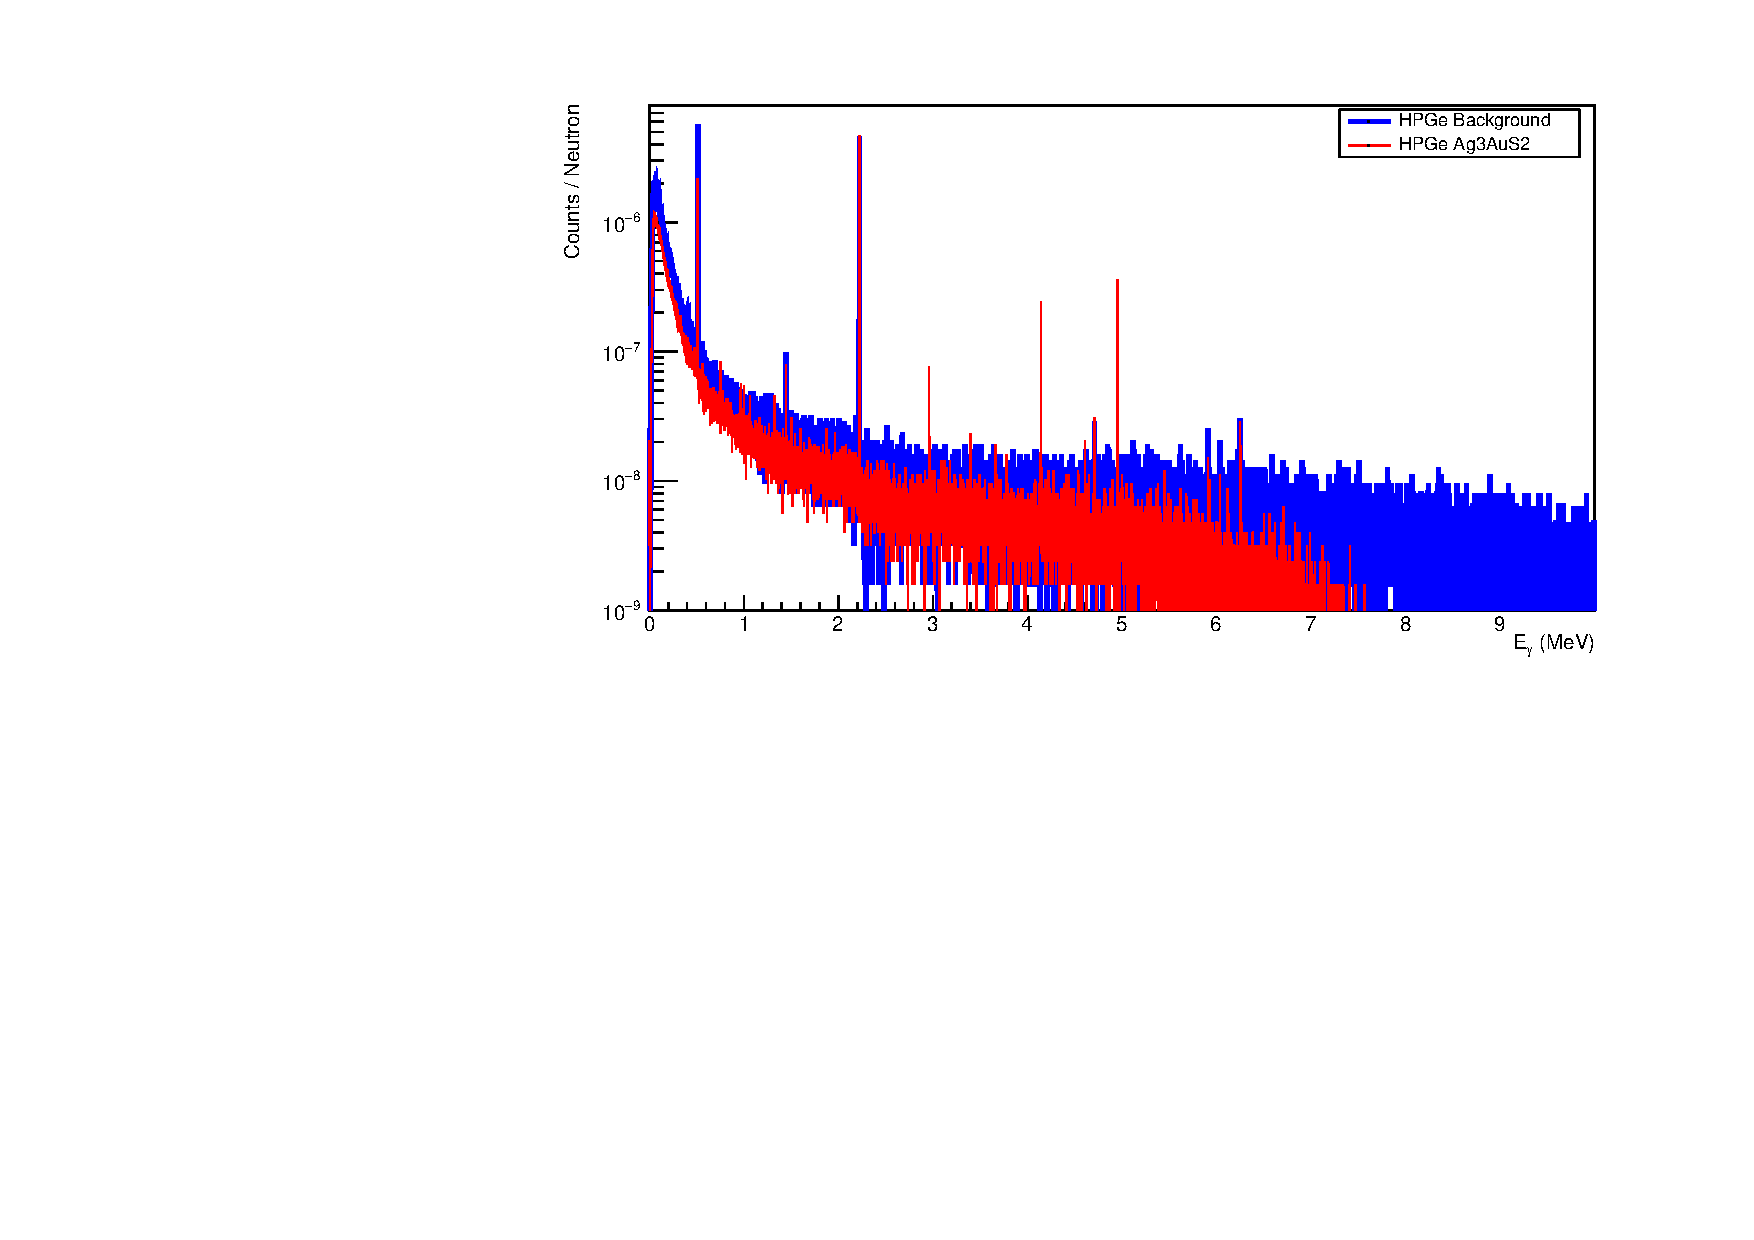
\includegraphics[width=1\textwidth]{res/Ag3AuS2_8_5MeVFonClasic.pdf}
	\caption{Червона - лінія спектру, набраного за опромінення нейтронами 8.5 МеВ}
	\label{ris:Ag3AuS28_5MeV}	
\end{figure} 
\begin{figure}[h!]
	%\vspace{-10pt}
	\centering 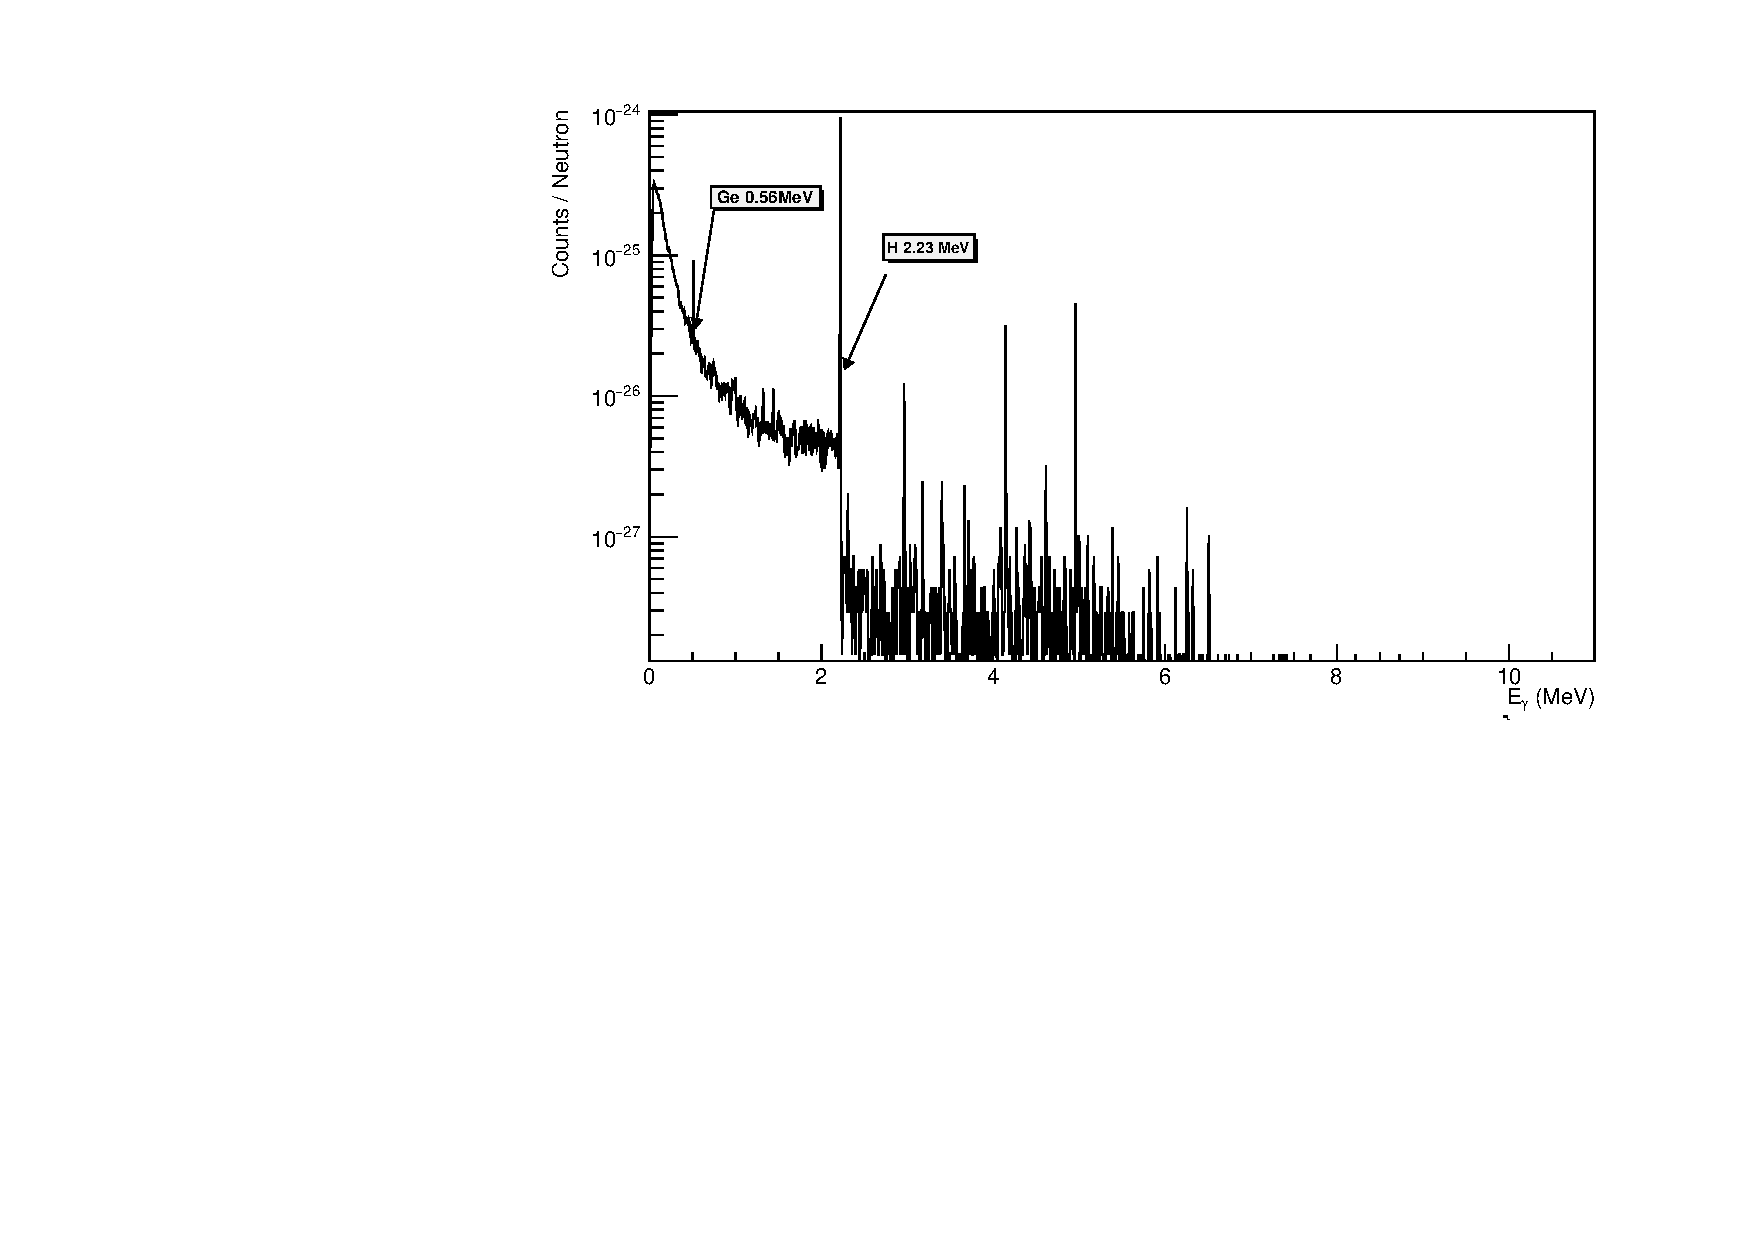
\includegraphics[width=1\textwidth]{res/AuAgS28MeV.pdf}
	\caption{Червона - лінія спектру, набраного за опромінення нейтронами 8.5 МеВ}
	\label{ris:Ag3AuS22_8MeV}	
\end{figure}
\begin{figure}[!]
	%\vspace{-10pt}
	\centering 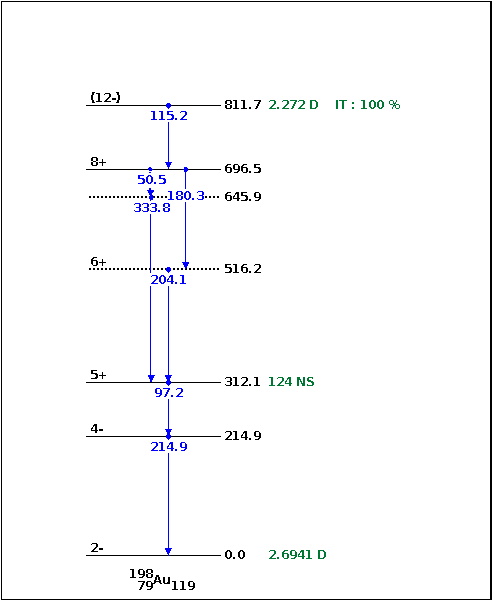
\includegraphics[width=1\textwidth]{images/au198levels.png}
	\caption{$Au^{198}$ Рівень $J\pi 12-$} 
	\label{ris:Au198Level12-}	
\end{figure} 
\begin{figure}[!]
	%\vspace{-10pt}
	\centering 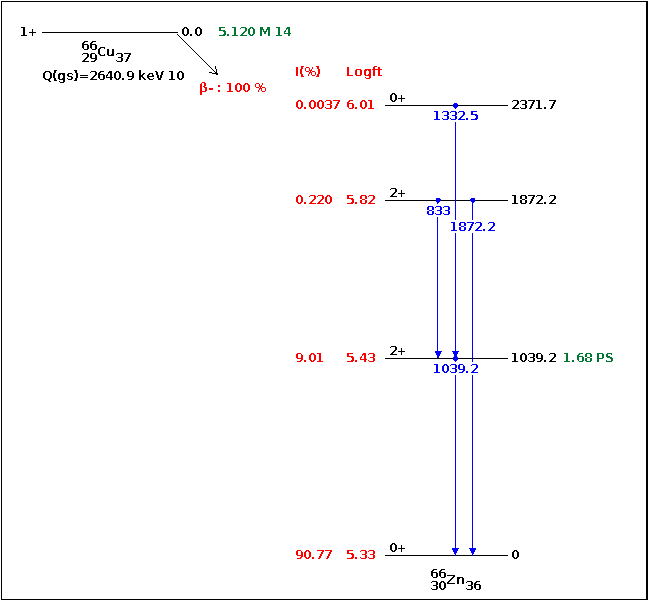
\includegraphics[width=1\textwidth]{images/cu66lbetadecay.png}
	\caption{$Cu^{66}_{29}(,\beta^-\  \tilde{\nu})Zn^{66}_{30}$ Схема розпаду та збудженні рівні $Zn^{66}$} 
	\label{ris:ZnLevels-}	
\end{figure} 

\pagebreak
\newpage	
%literature
\addcontentsline{toc}{section}{Література}
\begin{thebibliography}{}
	
%	\comment{кометар: це джерело звідки були взяті розміри детектора}  
	\bibitem{1} \textit{R.M. Keyser and T.R. Twomey} - Extended Source Sensitivity and Resolution Comparisons of Several HPGe Detector Types with Low-energy Capabilities 
	\bibitem{1} \textit{Aatos Heikkinen, Nikita Stepanov Helsinki Institute of Physics, P.O. Box 64, FIN-00014 University of Helsinki, Finland Johannes Peter Wellisch CERN, Geneva, Switzerland} - Bertini intra-nuclear cascade implementation in Geant4 
	\bibitem{1} \textit{Ю.В. Сереткин, Г.А. Пальянова Институт геологии и минералогии им. В.С. Соболева СО РАН} - ИЗОМОРФНОЕ ЗАМЕЩЕНИЕ СЕРЫ СЕЛЕНОМ И МОРФОТРОПНЫЙ ПЕРЕХОД В РЯДУ $Ag_3Au(Se,S)_2$ 	
	\bibitem{1} \textit{В. М. Округин1, А. У. Ким} О рудах Асачинского золото-серебряного месторождения
	(Южная Камчатка)
	\bibitem{1} \textit{Омельчук О.В., Загнітко В.М., Курило М.М.}ПОШУКИ ТА РОЗВІДКА РОДОВИЩ КОРИСНИХ КОПАЛИН КИЇВСЬКИЙ НАЦІОНАЛЬНИЙ УНІВЕРСИТЕТ ІМЕНІ ТАРАСА ШЕВЧЕНКА Навчально-науковий інститут «Інститут геології»
	\bibitem{1} \textit{Experimental Nuclear Reaction Data}
	\bibitem{1} \textit{O. A. Wasson, R. E. Chrien, M. R. Bhat, M. A. Lone, and M. Beer} $Au^{197}(n, \gamma)Au^{198}$ Reaction Mechanism 
	\bibitem{1} \textit{	I.A.Kondurov, A.I.Egorov, M.Kaminker, E.M.Korotkikh, A.M.Nikitin}  Neutron capture cross sections measurements for Co58m, Cu64, and Sc46
	\bibitem{1} \textit{ Geant4 Collaboration } Book For Application Developers
	Release 10.3
	\bibitem{1} \textit{ Alexander Howard, Gunter Folger, Jose Manuel Quesada, Vladimir Ivanchenko} Validation of Neutrons in Geant4 Using TARC Data - production, interaction and transportation

\end{thebibliography}

\end{document}
